\documentclass[a4paper, 12pt, oneside]{book}
\usepackage[utf8]{inputenc}
\usepackage[Lenny]{fncychap} % fancy chapter style (many more available, like Sonny, Bjarne, etc)
\ChNameVar{\Large\rm\bfseries} % Set name to serif, bold
\usepackage{color, xcolor} %edit e.g. text colors

\usepackage{titlesec}

\usepackage{xfrac}
\usepackage{cancel}
% Section: Sans-serif, Large, Bold, Dark Blue with an elegant underline
\titleformat{\section}
  {\normalfont\Large\bfseries}
  {\thesection}{1em}{}[{\vspace{0.2ex}\titlerule[0.8pt]}]

% Subsection: Sans-serif, large, bold, Dark Blue
\titleformat{\subsection}
  {\normalfont\large\bfseries}
  {\thesubsection}{1em}{}

% Subsubsection: Sans-serif, normal size, italic, Dark Blue
\titleformat{\subsubsection}
  {\normalfont\normalsize\itshape}
  {\thesubsubsection}{1em}{}
\usepackage{fancyhdr} %to customize the headers
\fancyhead{\nouppercase}
\usepackage[lmargin=1in, rmargin=1in, tmargin=1.5in, bmargin=1.3in]{geometry} %sets the margins for the pages
\setcounter{tocdepth}{3} %table of contents number depth for subsections (3 = x.x.x.x)
\setcounter{secnumdepth}{4} %numbering depth for headers for subsections in the text(4 = x.x.x.x)
\usepackage{url} %to include urls
\usepackage{lipsum}
\usepackage{listings} %include this if you want to include code in the thesis
\usepackage{amsmath,amssymb} %mathematical package
\usepackage[per-mode=symbol]{siunitx} %includes SI-units
\usepackage[bf]{caption} %makes float captions bold
\usepackage{array, booktabs} %to make better tables
\usepackage{graphicx} %to include graphics
\usepackage{float} %to include floats
\usepackage[export]{adjustbox} %to adjust floats
\usepackage{subcaption}
\usepackage{chngcntr} %will make it possible to change the counter for tables, figures etc. such as below
\usepackage{nicefrac} %to include nice fractions
%\counterwithin{figure}{section} %change counter for figures within sections (also possible to choose for each chapter
%\counterwithin{table}{section} %change counter for tables within sections
\usepackage{hyperref} %Adding internal links in you document
\usepackage{bookmark}
\usepackage{tikz-feynman} %to include feynman diagrams
\usepackage{tikz} %to include tikz figures
\usepackage{pgf} %to include pgf figures
\usepackage[spanish]{babel} %to include different languages, e.g. for captions

\hypersetup{
    colorlinks,
    citecolor=black,
    filecolor=black,
    linkcolor=black,
    urlcolor=black
}

% Define journal abbreviations
\def\aj{AJ}
\def\apj{ApJ}
\def\apjl{ApJL}
\def\apjs{ApJS}
\def\aap{A\&A}
\def\mnras{MNRAS}
\def\nat{Nature}
\def\prl{Phys. Rev. Lett.}

\usepackage[backend = biber,
            natbib = true,
            style = authoryear,
            maxcitenames = 2,
            ]{biblatex}
\addbibresource{bibliography.bib}
\usepackage{comment}
\usepackage{afterpage}
%\usepackage[version=4]{mhchem}

\newcommand\myemptypage{
    \null
    \thispagestyle{empty}
    \addtocounter{page}{-1}
    \newpage
    } %sets new page command to insert an empty page without adding to the page counter or having a page number

    \makeatletter
    \renewcommand*{\@makechapterhead}[1]{%
      \vspace*{0\p@}%
      {\parindent \z@ \raggedright \normalfont
        \ifnum \c@secnumdepth >\m@ne
          \if@mainmatter%%%%% Fix for frontmatter, mainmatter, and backmatter 040920
            \DOCH
          \fi
        \fi
        \interlinepenalty\@M
        \if@mainmatter%%%%% Fix for frontmatter, mainmatter, and backmatter 060424
          \DOTI{#1}%
        \else%
          \DOTIS{#1}%
        \fi
      }}
    % For the case \chapter*:
    \renewcommand*{\@makeschapterhead}[1]{%
      \vspace*{10\p@}%
      {\parindent \z@ \raggedright
        \normalfont
        \interlinepenalty\@M
        \DOTIS{#1}
        \vskip 40\p@
      }}
    \makeatother

\begin{document}

\newgeometry{top=2.5cm, bottom=2.5cm, left=2.5cm, right=2.5cm}
\begin{titlepage}
\begingroup
\renewcommand{\huge}{\fontsize{20.74}{25}\selectfont}
\renewcommand{\Large}{\fontsize{14.4}{18}\selectfont}

\newcommand{\HRule}{\rule{\linewidth}{0.5mm}}
\center 

\begin{figure}[t]
    \centering
    
\includegraphics[width=0.85\textwidth]{portada/logo_facultad.png}
\end{figure}
\hspace{2cm}

\textbf{\Huge Máster en Física Avanzada}\\[0.7cm]
\huge Especialidad Astrofísica\\[0.7cm] 

\begin{figure}[H]
    \centering
    
\includegraphics[width=0.3\textwidth]{portada/logo_uv.png}
\end{figure}
\hspace{1cm}

\textbf{\Huge Trabajo Fin de Máster}\\[0.3cm]
\HRule \\[1.5cm]
{ \huge \bfseries Estudio Astrosismológico de Blue Stragglers en el contexto de la misión HAYDN}\\[2.5cm]

\huge Pau Verdeguer Blom-Dahl\\[0.7cm]

\begin{minipage}[t]{0.45\textwidth}
    \begin{flushleft} 
    \end{flushleft}
\end{minipage}
\begin{minipage}[t]{0.52\textwidth}
    \begin{flushright} \Large
    {Tutores:} 
    Andrés Moya Bedón, Giovanni M. Miurouh \\ [0.5cm]

    \textit{Curso académico 2025/26}
    \end{flushright}
\end{minipage}

\vfill

\endgroup
\end{titlepage}
\restoregeometry

% The pre-chapters
\chapter*{Resumen} %pre-chapters should not be numbered, hence the "*"
\pagenumbering{roman} %introductory pages should be roman
\setcounter{page}{1}
\addcontentsline{toc}{chapter}{\protect\numberline{}Resumen} %add the chapter to the table of contents, this is not automatically added when creating unnumbered chapters (*). Add it in a chapter style, and keep all chapters on the same numberline indent regardless of number or not on the chapter

Las \textit{Blue Stragglers} son estrellas que aparecen más calientes y luminosas que el \textit{turn-off point} de su cúmulo estelar, aparentando haber ``rejuvenecido''. Para explicar su origen existen dos hipótesis: la \textit{hipótesis aislada} y la \textit{hipótesis de transferencia de masa binaria}. Ambos escenarios producen estrellas en idénticas posiciones del diagrama HR, lo que impide diferenciarlas con técnicas observacionales convencionales. Este trabajo evalúa si la astrosismología puede discriminar entre ambas historias evolutivas, en el contexto de la propuesta de misión espacial HAYDN de la ESA.

Se ha simulado la formación de una Blue Straggler mediante transferencia de masa empleando el código MESA, a partir de un sistema binario con una donante de $2.0\,M_\odot$ y una acretora de $1.0\,M_\odot$. El resultado es una estrella rejuvenecida de $1.82136\,M_\odot$ con un perfil de composición química distinto al de una estrella simple. Las frecuencias de oscilación (modos $l=0,1,2$; $n_{pg} \in [-10,10]$) de esta Blue Straggler y de estrellas de referencia de masa similar se han calculado con el código GYRE, comparándolas en 7 puntos significativos de la secuencia principal.

Los resultados muestran diferencias entre ambos escenarios. Los indicadores más sensibles son los modos no radiales ($l\neq0$): en la gran separación ($\Delta\nu$), los modos $l=2$ alcanzan diferencias de hasta ${\sim}\,2.5\,\text{ciclos\,día}^{-1}$ al final de la secuencia principal. La pequeña separación ($\delta\nu_{02}$) y las frecuencias individuales de los modos g muestran diferencias del mismo orden. Se estima un tiempo de integración mínimo de ${\sim}\,142$ días para resolver las diferencias más pequeñas, compatible con las campañas de observación previstas por HAYDN.

El principal obstáculo para la aplicabilidad observacional es la identificación inequívoca de los modos de oscilación en estrellas $\delta$~Scuti, región del diagrama HR donde se ubican las Blue Stragglers, dada la complejidad de su espectro de frecuencias.

\bigskip
\noindent\textbf{Palabras clave:} astrosismología, Blue Stragglers, oscilaciones estelares, MESA, GYRE, transferencia de masa binaria, gran separación, pequeña separación, HAYDN.
 %insert the chapter text from the files

%add an empty non-counted page by the command below in order to get the first chapter on the left hand side, if needed (check your page number so that the first chapter is on an odd page)

\chapter*{Prefacio}
\addcontentsline{toc}{chapter}{\protect\numberline{}Prefacio} 

El estudio de la evolución estelar constituye uno de los pilares fundamentales de la astrofísica moderna. Tradicionalmente, los modelos de evolución de estrellas aisladas han sido un marco robusto para comprender el ciclo de vida de los astros. Sin embargo, la vasta población de sistemas binarios y múltiples en el universo introduce escenarios complejos que desafían las aproximaciones más idealizadas. Entre estos fenómenos, las blue stragglers representan uno de los mayores enigmas: estrellas que, pese a la posición del punto de desvío de su cúmulo estelar, parecen haber encontrado una ``fuente de la eterna juventud''.

Este Trabajo de Fin de Máster nace con el propósito de arrojar luz sobre los mecanismos internos que gobiernan a estas estrellas mediante el uso de la astrosismología, una muy potente herramienta capaz de indagar en interior estelar a través de sus modos de oscilación. Tomando como base de simulación los códigos MESA y GYRE, esta investigación se sumerge en el modelado bidimensional de la estructura y pulsación de estos productos de la evolución binaria.

El alcance de este trabajo no se limita, sin embargo, a la exploración teórica abstracta. La pertinencia y el impacto de este análisis se enmarcan y justifican dentro del contexto científico de la propuesta de misión espacial HAYDN (High-precision AsteroseismologY in DeNse stellar fields) de la Agencia Espacial Europea (ESA). Diseñada para operar en campos estelares densos y cúmulos jóvenes mediante fotometría de altísima precisión, HAYDN promete revolucionar nuestra comprensión de la física estelar. Los modelos teóricos desarrollados en esta tesis pretenden servir como un primer paso de contribución al marco preparatorio de dicha misión, demostrando el potencial que la astrosismología tiene para revelar la historia evolutiva y estructural de este tipo de estrellas.

Afrontar este proyecto ha supuesto no solo un reto intelectual en el ámbito de la astrofísica estelar, sino también un profundo aprendizaje en el desarrollo de herramientas computacionales, la modificación de entornos de simulación numérica y la interpretación de espectros de frecuencia pulsacionales. Es el resultado de meses de dedicación orientados a un horizonte donde la teoría astrosismológica y el futuro de la exploración espacial europea se dan la mano.

\tableofcontents


%%%%%%%%%%%%%%%%%%%%%%%%%%%%%%%%%%%%%%%%%%%%%%%%%%%%%%%%
%Customize the layout of the main content of your thesis

\pagestyle{fancy} %set customized page style for header
%\fancyhf{} %clear header and footer fields
\renewcommand{\headrulewidth}{0pt} %set to no rule
%\fancyhead[LO, RO]{\thepage} %set the page number at left for even, right for odd pages
\fancyhead[L]{\leftmark} %set the chapter name at right for even, left for odd pages
%is is possible to design the header with the chapter as you wish, e.q. only the chapter or only the name, all lowercase instead etc.
%you could also design the footer if you wish, for example:

\setlength{\headheight}{14.49998pt} %set the header height


%%%%%%%%%%%%%%%%%%%%%%%%%%%%%%%%%%%%%%%%%%%%%%%%%%%%%%%%
%main content 

\pagenumbering{arabic}

\chapter{Introducción}

La astrosismología es el estudio de las oscilaciones estelares mediante el análisis de los cambios que estas provocan en la luz de las estrellas \citep{ChristensenDalsgaard2019}. Dichos cambios se manifiestan como pequeñas variaciones en el brillo (fotometría) o como desplazamientos en las líneas espectrales debido al efecto Doppler (espectroscopía), y permiten obtener información acerca de la estructura interior, composición química e historia evolutiva de las estrellas.

Estas oscilaciones corresponden a modos propios de vibración atrapados en el interior de la estrella. El análisis de estos modos permite determinar con precisión los gradientes de densidad, la rotación interna del núcleo y la extensión de las zonas de mezcla convectiva, entre otros, proporcionando una visión de la estructura interna que la fotometría clásica no puede dilucidar \citep{ChristensenDalsgaard2019}.

En presente trabajo tiene como objetivo establecer, en el marco de la propuesta de misión HAYDN de la ESA \citep{haydn_mission_proposal_2026}, una distinción de estrellas con diferentes historias evolutivas mediante la astrosismología. En concreto, se estudiarán las denominadas \textit{Blue Stragglers} para comprobar si la astrosismología puede diferenciarlas de estrellas con historias evolutivas distintas que se encuentren en la misma posición aparente en el diagrama HR.

\section{\textit{Blue Stragglers}}

Los cúmulos estelares resultan ser de gran importancia a la hora de probar modelos teóricos de evolución estelar, puesto que permiten comparar sus predicciones con las observaciones. Esto se debe a que se asume que las estrellas de un mismo cúmulo se formaron alrededor del mismo momento y con una composición química muy similar (provienen de la misma nube de gas y polvo). Al asumir esto como verdadero, se puede estudiar en detalle cómo la masa inicial de una estrella determina su evolución a lo largo del tiempo sin la interferencia de otros parámetros desconocidos \citep{TASC8KASC15AbstractBooklet}.

Esta homogeneidad permite modelar la población de un cúmulo mediante el uso de isócronas: curvas teóricas en el diagrama HR que representan las posiciones de estrellas de la misma edad y composición química, pero con diferentes masas iniciales. A medida que el cúmulo envejece, las estrellas más masivas agotan el hidrógeno en su núcleo y abandonan la secuencia principal. El punto preciso del diagrama donde se produce esta transición se conoce como el ``\textit{turn-off point}'', y permite estimar la antigüedad de un cúmulo en concreto \citep{wang2024bluestragglerstars}.

\begin{figure}[H]
  \centering
  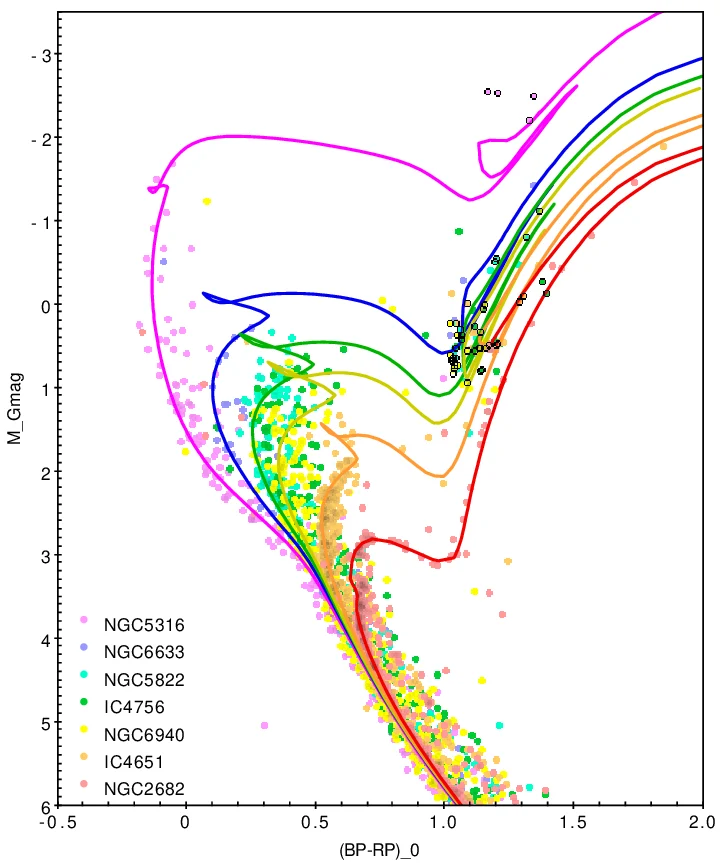
\includegraphics[width=0.8\textwidth]{Imagenes/HR_isoch.png}
  \caption{Diagrama HR para distintos cúmulos estelares con las isócronas de mejor ajuste superpuestas. Puede apreciarse el ``\textit{turn-off point}'' en diferentes posiciones dependiendo de la edad del cúmulo. Cuanto más a la derecha se encuentra este punto, más antiguo es el cúmulo. Imagen tomada de \citet{santrich_2022}.}
  \label{fig:hr_diagram}
\end{figure}

No obstante, al elaborar este tipo de diagramas, a menudo se observan una serie de anomalías que escapan a la explicación de los modelos estelares evolutivos simples. Un ejemplo de ello son las \textit{Blue Stragglers}, estrellas más calientes y luminosas que el resto de estrellas de un mismo cúmulo, y que, de alguna manera, parecen haber ``rejuvenecido'' (ya que se encuentran arriba y a la izquierda del \textit{turn-off point} de su cúmulo) \citep{wang2024bluestragglerstars}. Un ejemplo de este tipo de estrellas se puede apreciar en la Figura \ref{fig:hr_diagram_bss}.

\begin{figure}[H]
  \centering
  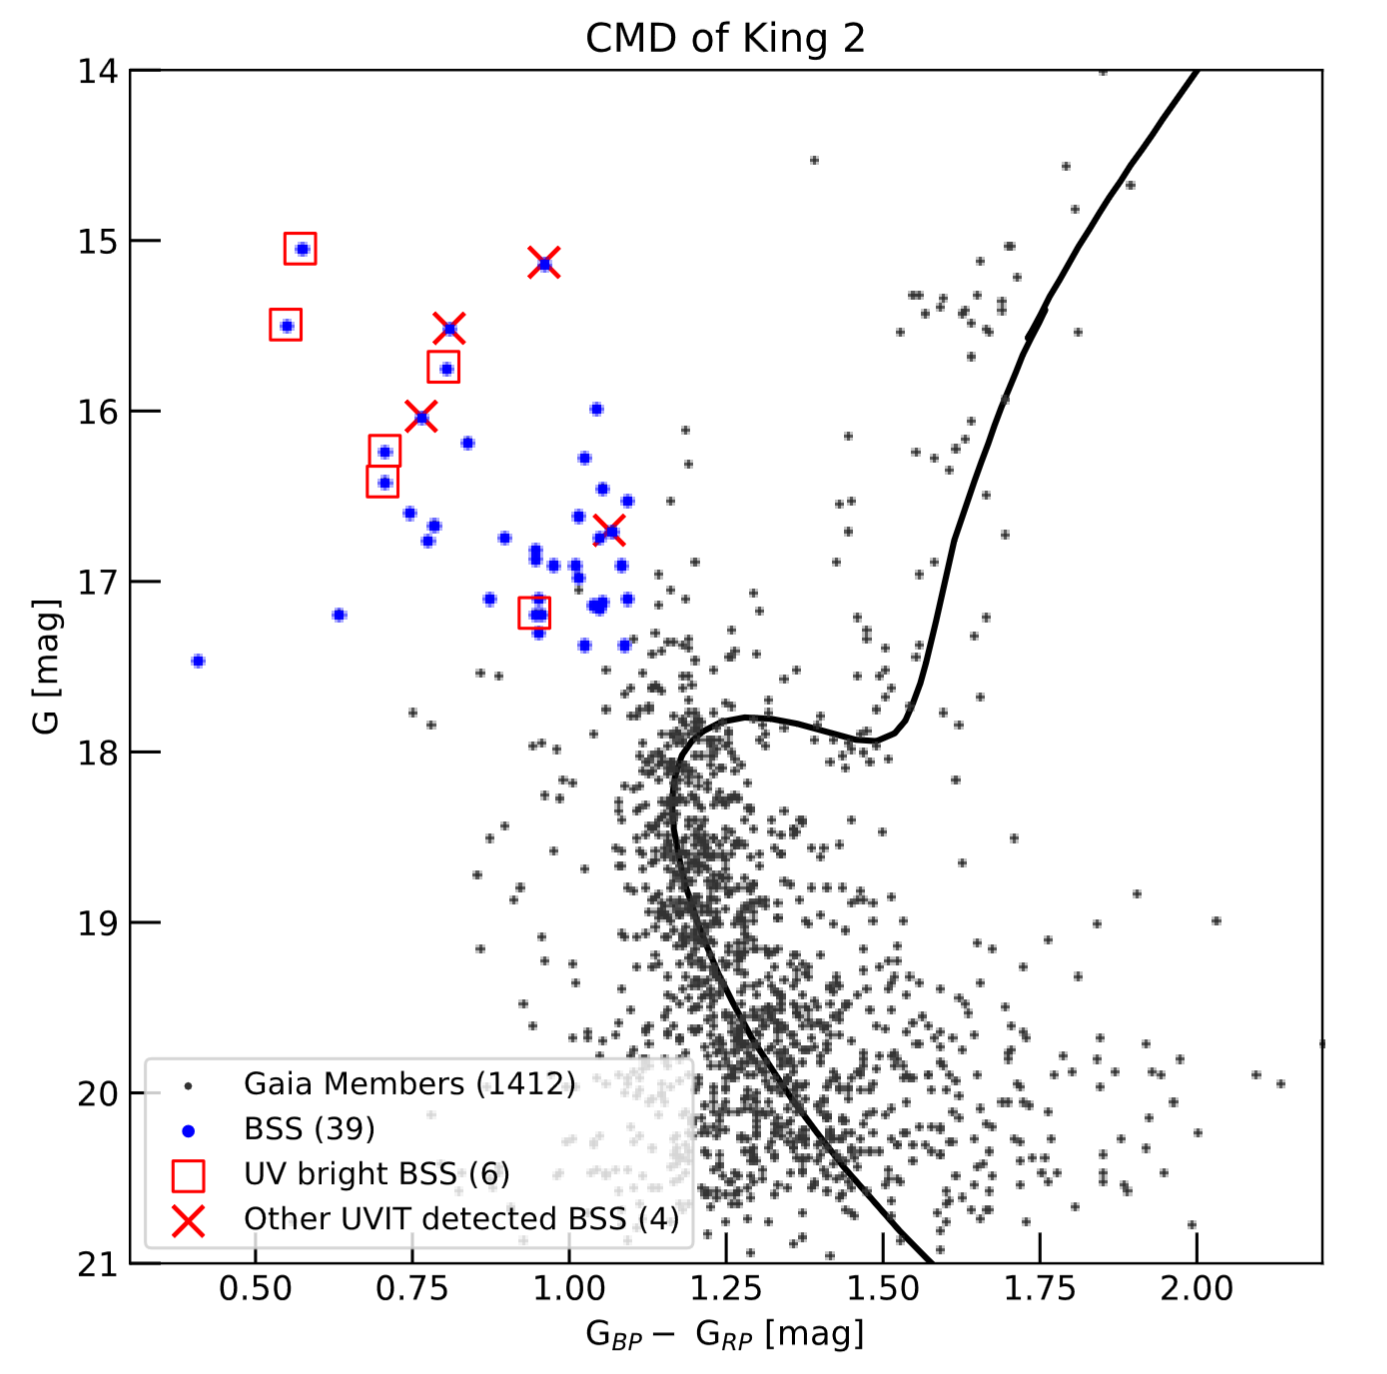
\includegraphics[width=0.65\textwidth]{Imagenes/HR_BSS.png}
  \caption{Diagrama HR de los miembros del cúmulo King 2. Las estrellas en azul conforman el grupo de \textit{Blue Stragglers} del cúmulo. La isócrona de mejor ajuste del cúmulo tiene los parámetros $\log(\text{edad}) = 9.7$, $\mathrm{[M/H]} = -0.4$, $\text{DM} = 13.8$ y $E(B-V) =0.45$. Figura tomada de \citet{Jadhav_2021}.}
  \label{fig:hr_diagram_bss}
\end{figure}

Frecuentemente, este tipo de estrellas se ubican en una zona del diagrama HR correspondiente a tres tipos de estrellas pulsantes: $\delta$ Scuti, $\gamma$ Doradus, y SX Phoenicis \citep{Kurtz2022, 10.3389/fspas.2022.952296}. Las $\delta$ Scuti oscilan en la zona correspondiente a modos p y g de bajo orden (alrededor del fundamental radial), las $\gamma$ Doradus oscilan en la zona correspondiente a modos g de alto orden (bajas frecuencias) y las SX Phoenicis, principalmente, en la zona correspondiente al fundamental radial y primer sobretono ($n_{\mathrm{pg}} = 0, 1$) \citep{Handler_2009,10.3389/fspas.2022.952296}. En el Capítulo 2 se profundizará acerca de estos modos de oscilación. Una imagen de la distribución de tipos de estrellas pulsantes en el diagrama HR se puede apreciar en la Figura \ref{fig:hr_diagram_pulsating_stars}.

\begin{figure}[t]
  \centering
  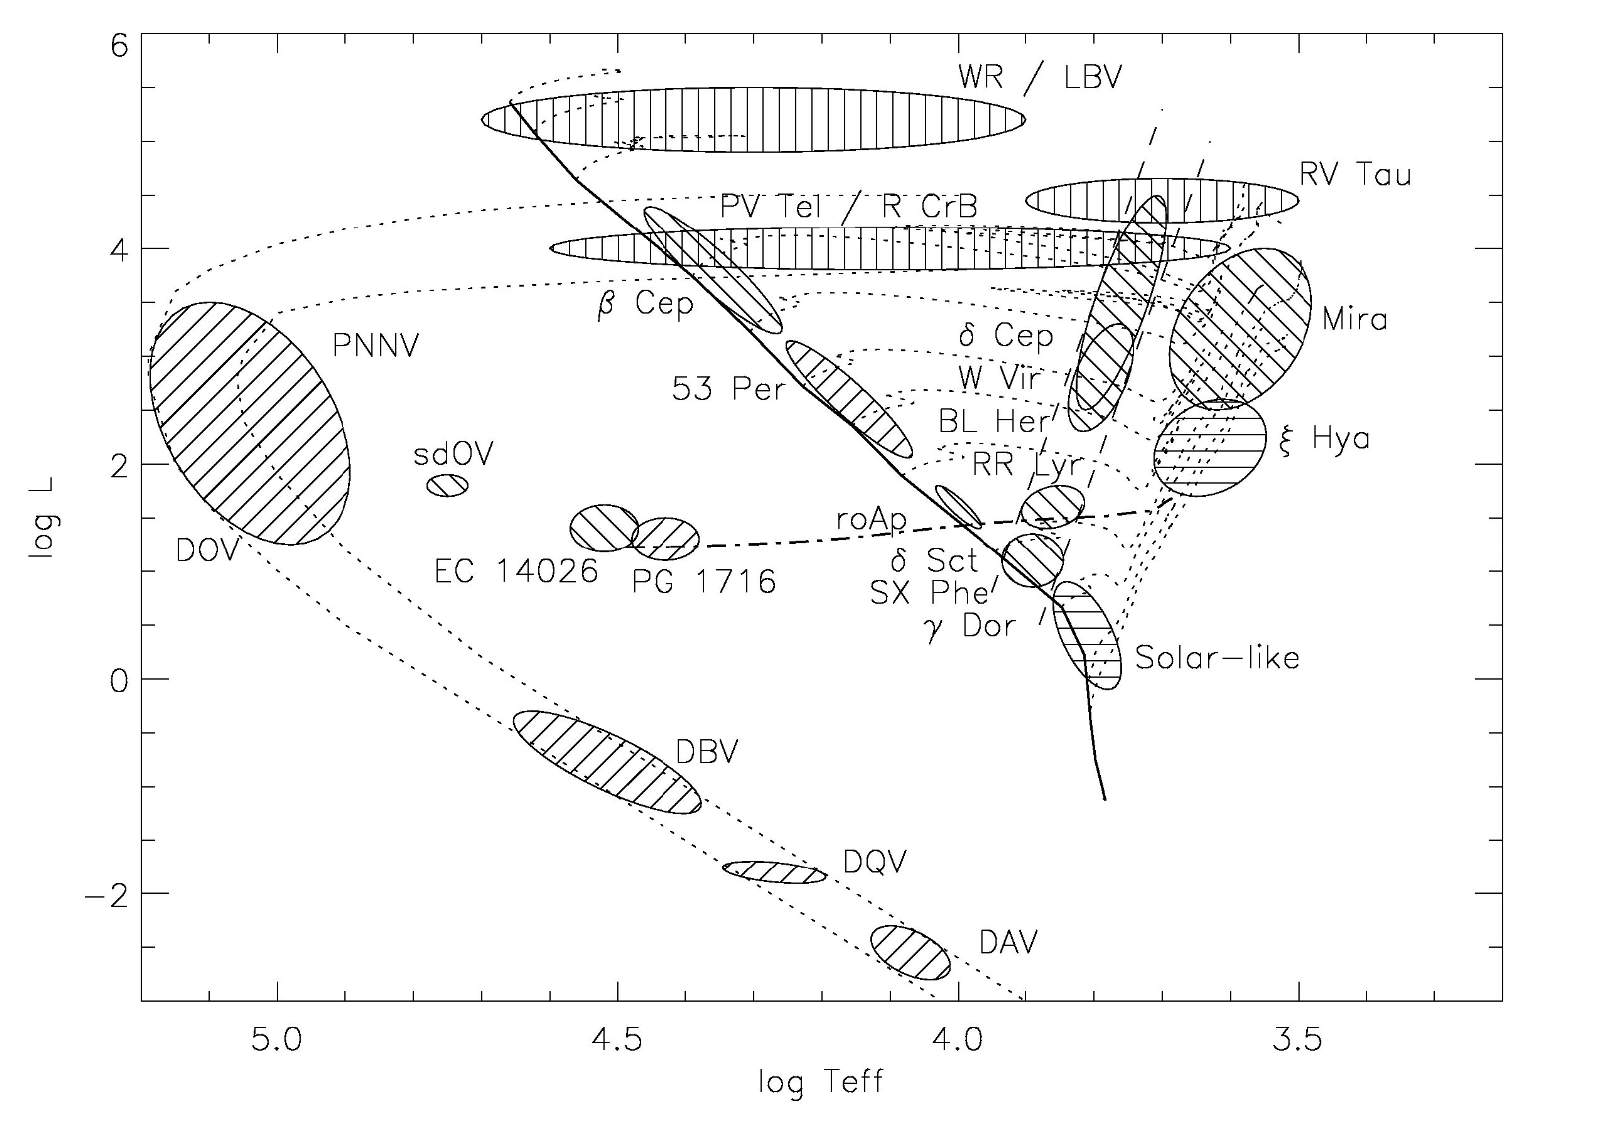
\includegraphics[width=\textwidth]{Imagenes/HR_Pulsating.png}
  \caption{Distribución de tipos de estrellas pulsantes en el diagrama HR. Figura tomada de \citet{2008CoAst.157..240J}.}
  \label{fig:hr_diagram_pulsating_stars}
\end{figure}

Existen diversas hipótesis para explicar la existencia de este tipo de estrellas. Por ejemplo: la transferencia de masa en sistemas binarios, las fusiones binarias, las colisiones estelares y la evolución atípica de estrellas individuales \citep{wang2024bluestragglerstars}. En este trabajo se busca diferenciar dos de ellas: la \textit{hipótesis aislada} y la \textit{hipótesis de transferencia de masa binaria}, mediante la astrosismología.

El modelo teórico de evolución estelar más simple asume una evolución aislada, es decir, que la estrella no interactúa con otros objetos celestes. En este caso, la explicación de la existencia de estas \textit{blue stragglers} es que son estrellas de una masa inicial alta, las cuales (por alguna razón desconocida) se formaron mucho más tarde que el resto de estrellas de su cúmulo. Esta es la \textit{hipótesis aislada}, y constituye nuestro modelo comparativo de control (\textit{baseline}).

La alternativa es que estas \textit{blue stragglers} se encuentren en sistemas binarios con otro objeto, el cual ha transferido parte de su material a la estrella (inicialmente con menor masa), provocando que esta se vuelva más masiva y caliente. Esta es la \textit{hipótesis de transferencia de masa binaria} \citep{wang2024bluestragglerstars}.

Estas dos hipótesis no pueden ser diferenciadas únicamente utilizando el diagrama HR. Dos estrellas con historias evolutivas completamente distintas pueden ubicarse en la misma posición, ocultando sus diferencias internas. Debido a ello se recurre a la astrosismología. Al estudiar las pulsaciones de dos estrellas en la misma posición pero con historias evolutivas distintas, se espera encontrar diferencias cuantificables en sus frecuencias de oscilación que permitan discernir cuál de las dos hipótesis es la correcta.

Esto lleva a la siguiente pregunta: ¿Qué tipo de observaciones astrosismológicas son necesarias para poder diferenciar entre estas dos hipótesis? Aquí es donde entra en juego la misión HAYDN.

\section{HAYDN}
La propuesta de misión HAYDN (acrónimo en inglés de High-precision AsteroseismologY in DeNse stellar fields) \citep{HAYDN} es una propuesta de misión espacial de clase media europea concebida en el marco del programa científico a largo plazo Voyage 2050 de la Agencia Espacial Europea. Actualmente, HAYDN se encuentra en fase de evaluación competitiva frente a otras propuestas para la misión M8 de la ESA, luego de haber superado la primera fase de selección y tener una buena base tras su evaluación inicial en la anterior convocatoria (M7). El proyecto está liderado por Andrea Miglio (Universidad de Bolonia) como Investigador Principal, y cuenta con un extenso consorcio internacional de más de 200 científicos (entre los que destaca Andrés Moya Bedón, tutor del presente proyecto, quien se desempeña como Investigador Principal de dicha misión en España y Co-Investigador Principal a nivel global.)

El objetivo de HAYDN es obtener series temporales fotométricas de alta precisión, alta cadencia y larga duración para grandes muestras de estrellas situadas en entornos estelares densos y ``controlados'', como son los cúmulos estelares abiertos (p. ej. $\chi$ y h Persei), cúmulos de edad intermedia (p. ej. M67), cúmulos globulares antiguos (p. ej. 47 Tuc y NGC 6397) y otras estructuras complejas, como son el bulbo de la Vía Láctea y Omega Centauri, hipotético remanente del cúmulo central de una galaxia absorbida por la Vía Láctea hace miles de millones de años \citep{Bekki_2003, haydn_mission_proposal_2026}.

En la década pasada, diversas misiones como CoRoT, Kepler y TESS han permitido obtener resultados con un alto valor científico en el marco de la astrosismología \citep{HAYDN,haydn_mission_proposal_2026, TASC8KASC15AbstractBooklet, IAUCommissionG4Report2024}. Sin embargo, el propósito de dichas misiones no era el estudio de las oscilaciones estelares, sino el de detectar exoplanetas a través del método de tránsitos en estrellas brillantes del campo galáctico. El problema que presentan para la toma de datos astrosismológicos en campos estelares densos es que emplean instrumentos con tamaños de píxel muy grandes en el cielo (TESS, por ejemplo, tiene píxeles que abarcan $20''$), y las \textit{Point-Spread-Functions} (PSFs) de las estrellas no son suficientemente pequeñas \citep{HAYDN,haydn_mission_proposal_2026}.

Esto impide tomar series fotométricas de estrellas individuales cuando estas se encuentran en campos altamente poblados, como son los cúmulos estelares densos y el centro galáctico debido a la severa contaminación por el solapamiento de la luz de estrellas vecinas. HAYDN soluciona esto empleando una escala del píxel del orden de $0.25''$ y un campo de visión más concentrado ($\lesssim 1^\circ$). Esto le permite resolver estrellas densamente agrupadas.

\begin{figure}[htpb]
  \centering
  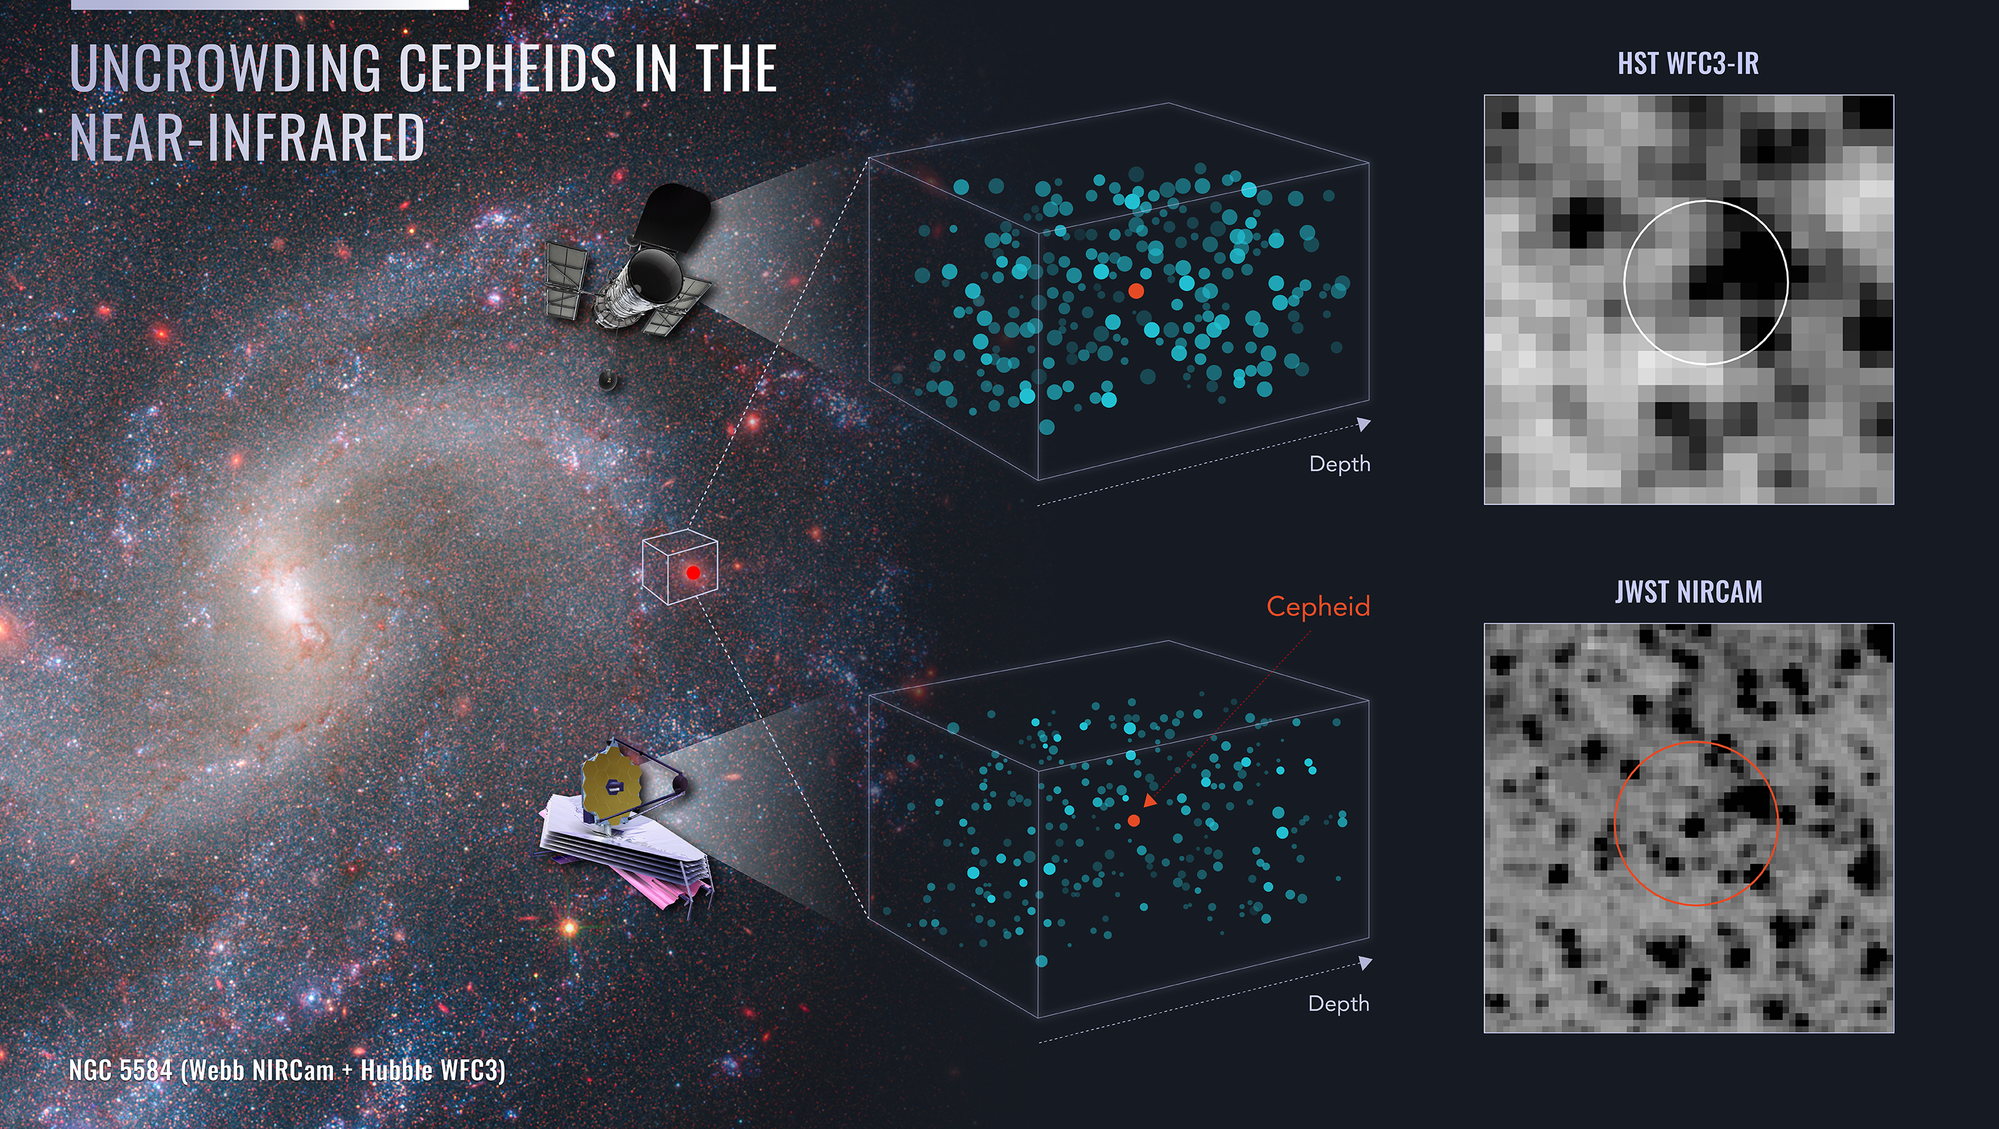
\includegraphics[width=0.8\textwidth]{Imagenes/cepheids.png}
  \caption{Imagen que muestra la galaxia NGC 5584. La visualización ilustra cómo el telescopio Webb (NIRCam) logra separar una estrella Cefeida (punto naranja) de la multitud de estrellas de fondo (puntos azules), una distinción que la menor resolución del Hubble (WFC3-IR) en el infrarrojo cercano no permitía hacer con claridad, como se ve en los recuadros ampliados. Imagen tomada de \citet{NASAWebb2023Cepheids}}
\end{figure}
\subsection{Objetivos y Arquitectura}

HAYDN proporcionará datos asterosísmicos sin precedentes en poblaciones estelares químicamente homogéneas y con edades bien determinadas. Esto le permitirá resolver preguntas clave en astrofísica. Para ello, se estructura en objetivos centrales que pueden agruparse de la siguiente manera \citep{HAYDN,haydn_mission_proposal_2026}:

\begin{itemize}
  \item \textbf{Astrofísica estelar y sistemas planetarios:} Se busca obtener restricciones sísmicas directas sobre procesos físicos internos, transporte de momento angular y pérdida de masa, enfocándose en estrellas masivas ($10$ -- $15~M_\odot$) progenitoras de objetos compactos. Además, investigará cómo el entorno de los cúmulos densos y diversos afecta la formación y características de los exoplanetas.
  \item \textbf{Calibración fundamental y arqueología galáctica:} Utilizará cúmulos estelares para refinar modelos físicos y calibrar escalas cósmicas de distancia y edad, lo que permitirá caracterizar el historial de formación de poblaciones estelares en entornos complejos (como el bulbo galáctico y galaxias enanas).
\end{itemize}

Estos objetivos se consiguen mediante una doble estrategia: una Muestra de Alta Precisión (HPS) para inferencia sísmica profunda y una Muestra de Sondeo (SS) para características poblacionales amplias. Los objetivos incluyen cúmulos de referencia (M67, 47 Tuc, $\chi$+ h Persei y el complejo $\omega$ Centauri), abarcando edades desde 10 Myr hasta 13 Gyr y metalicidades desde $\mathrm{[Fe/H]} \approx +0.1$ hasta $-2.0$ \citep{haydn_mission_proposal_2026}.

\subsection{Arquitectura y Operaciones}

Para cumplir sus objetivos, la misión HAYDN operará desde el punto de Lagrange L2 durante 4 años (con posibilidad de extensión), garantizando observaciones continuas sin fluctuaciones térmicas ni eclipses. Su arquitectura preliminar contempla:

\begin{itemize}
  \item Un espejo primario de 1.37 m de diámetro (equivalente a 120 cm sin obstrucción) con diseño óptico de dos espejos y tres reflexiones y un campo de visión de alrededor de $1^\circ$.

  \item Campañas de observación de larga duración (3, 6, 9 y hasta 18 meses continuos) sobre campos específicos, indispensables para obtener la resolución frecuencial necesaria para detectar la fina estructura de modos de pulsación mezclados y medir perfiles de rotación.

  \item Una importante colaboración con otros proyectos espectroscópicos terrestres e instrumentos, como el futuro HRMOS y los datos de la misión Gaia, lo que permitirá incrementar drásticamente su valor científico.
\end{itemize}

\vspace{1cm}
Antes de simular los modelos estelares y evaluar su posible detección observacional, es necesario establecer el marco físico y matemático que rige las pulsaciones en los interiores estelares.
\chapter{Hidrodinámica y Oscilaciones Estelares}

\noindent Buena parte de la astrofísica estelar se sustenta bajo las ecuaciones de la hidrodinámica. Es la base matemática ideal para describir el gas del interior de las estrellas como un fluido continuo. En este capítulo, dichas ecuaciones se presentan, así como su formulación en el marco de la teoría de perturbaciones.

\section{Ecuaciones Básicas de la Hidrodinámica}
Las propiedades esenciales del gas estelar pueden especificarse como funciones de la posición y del tiempo. Estas propiedades incluyen la densidad local $\rho(\mathbf{r},t)$, la presión $p(\mathbf{r},t)$, la temperatura $T(\mathbf{r},t)$ (y/o cualquier otra cantidad termodinámica relevante) y la velocidad del fluido $\mathbf{v}(\mathbf{r},t)$. Aquí, $\mathbf{r}$ denota el vector posición con respecto a un punto de referencia en el espacio, correspondiéndose con lo que vería un observador en reposo. Esta descripción, pues, se conoce como la descripción \textit{Euleriana} del fluido. Otra descripción posible es la \textit{Lagrangiana}, en la cual un observador sigue el movimiento de un elemento de fluido a medida que se desplaza por el espacio. En este marco, un elemento de gas puede ser etiquetado por su posición inicial $\mathbf{r}_0$, y sus propiedades se describen como funciones de $\mathbf{r}_0$ y del tiempo $t$ (por ejemplo, $\mathbf{r}(\mathbf{r}_0,t)$).

\begin{figure}[htbp]
    \centering
    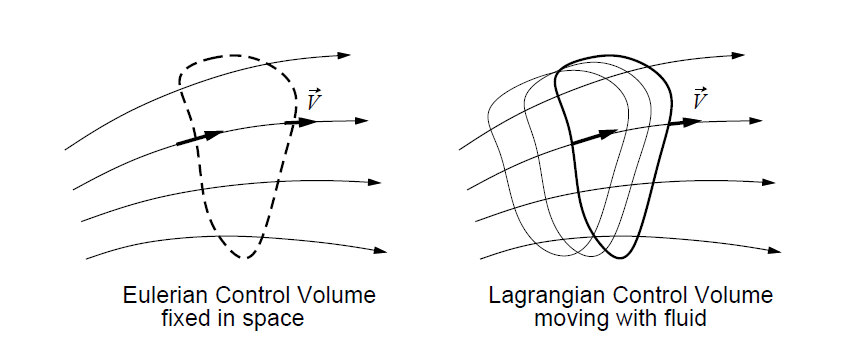
\includegraphics[width=\linewidth]{Imagenes/euler_vs_lagrange.png}
    \caption{La descripción Euleriana describe el flujo del fluido desde la perspectiva de un volumen fijo en el espacio. La descripción Lagrangiana describe el flujo del fluido desde la perspectiva de un elemento de fluido individual. Imagen tomada de \autocite{PhysicsStackExchange537111}}
\end{figure}

La derivada temporal de una cantidad $\phi$, observada desde un marco lagrangiano, es

\begin{equation}
\frac{d \phi}{d t} = \left( \frac{\partial \phi}{\partial t} \right)_{\mathbf{r}} + \nabla \phi \cdot \frac{d \mathbf{r}}{d t} = \frac{\partial \phi}{\partial t} + \mathbf{v} \cdot \nabla \phi, 
\end{equation}
notando que $\mathbf{v(\mathbf{r}, t)} = \frac{d \mathbf{r}}{d t}$.


La conservación de la masa en un fluido nos lleva a la ecuación de continuidad, que en la descripción Euleriana suele expresarse como
\begin{equation}
\frac{\partial \rho}{\partial t} + \nabla \cdot (\rho \mathbf{v}) = 0,
\label{eq:continuidad}
\end{equation}

dicha ecuación establece un balance entre la tasa de cambio de la densidad local y el flujo de gas a través de un cierto volumen. Si hubiera existido una fuente de masa en el sistema, dicho término aparecería en el lado derecho de esta ecuación.

La siguiente ecuación a tener en cuenta es la ecuación del momento, expresada como

\begin{equation}
    \rho \left( \frac{\partial \mathbf{v}}{\partial t} + \mathbf{v} \cdot \nabla \mathbf{v} \right) = -\nabla p + \rho \mathbf{g}
\end{equation}

donde $\mathbf{g} = - \nabla \Phi$ es el vector de aceleración gravitatoria. En este punto consideramos que la gravitatoria es la única fuerza externa que actúa sobre el fluido.

Podemos también en este punto escribir la ecuación de Poisson, que relaciona la densidad de masa con el potencial gravitatorio $\Phi$:

\begin{equation}
    \nabla^2 \Phi = 4 \pi G \rho,
\end{equation}

siendo $G$ la constante de gravitación universal.

Finalmente, es necesaria una relación termodinámica entre entre densidad y presión. Tenemos que

\begin{equation}
    \frac{d q}{d t} = \frac{d E}{d t} + p \frac{d V}{d t},
    \label{eq:primerprincipio}
\end{equation}
siendo $d q/d t$ la tasa de cambio de calor y $E$ la energía interna del gas por unidad de masa. $V = 1 / \rho$ es el volumen específico del gas. Podemos formular \eqref{eq:primerprincipio} utilizando \eqref{eq:continuidad}:

\begin{equation}
    \frac{d q}{d t} = \frac{d E}{d t} - \frac{p}{\rho^2} \frac{d \rho}{d t} = \frac{d E}{d t} + \frac{p}{\rho} \nabla \cdot \mathbf{v},
\end{equation}
y, utilizando relaciones termodinámicas, puede escribirse como
\begin{align}
    \frac{d q}{d t} &= \frac{1}{\rho (\Gamma_3 - 1)} \left(\frac{d p}{d t} - \frac{\Gamma_1 p}{\rho} \frac{d \rho}{d t}\right) \\
    &= c_p \left(\frac{d T}{d t} - \frac{\Gamma_2 - 1}{\Gamma_2}\frac{T}{p}\frac{d p}{d t} \right) \\
    &= c_V \left[\frac{d T}{d t} - (\Gamma_3 - 1)\frac{T}{\rho}\frac{d \rho}{d t} \right],
\end{align}

$c_p$ y $c_V$ son las capacidades caloríficas a presión y volumen constantes, respectivamente, y $\Gamma_1$, $\Gamma_2$ y $\Gamma_3$ son los índices adiabáticos del gas, definidos como:

\begin{equation}
\Gamma_1 = \left( \frac{\partial \ln p}{\partial \ln \rho} \right)_{ad}, \quad
\frac{\Gamma_2 - 1}{\Gamma_2} = \left( \frac{\partial \ln T}{\partial \ln p} \right)_{ad}, \quad
\Gamma_3 - 1 = \left( \frac{\partial \ln T}{\partial \ln \rho} \right)_{ad}.
\end{equation}

\subsection{Aproximación Adiabática}

Podemos considerar una ecuación de estado del gas simple, como la ecuación de estado de un gas ideal, que podemos expresar como

\begin{equation}
    p = \frac{\rho k_B T}{\mu m_u},
\end{equation}
donde $k_B$ es la constante de Boltzmann, $m_u$ es la unidad de masa atómica y $\mu$ es el peso molecular medio del gas. Además consideramos $\Gamma_1 = \Gamma 2 = \Gamma 3 = 5/3$. Considerando de nuevo la ecuación energética, esta puede escribirse como

\begin{equation}
\rho \frac{d q}{d t} = \rho \epsilon - \nabla \cdot \mathbf{F},
\end{equation}

donde $\epsilon$ es la tasa de generación de energía por unidad de masa y $\mathbf{F}$ es el flujo de energía. En el caso de que el gas sea completamente convectivo, podemos considerar que $\mathbf{F} = 0$. En este caso únicamente incluimos el flujo radiativo en la ecuación anterior.

En interiores estelares, el flujo radiativo viene dado por

\begin{equation}
    \mathbf{F} = - \frac{4 a \tilde{c} T^3}{3 \kappa \rho} \nabla T,
\end{equation}

siendo $a$ la constante de densidad de radiación, $\tilde{c}$ la velocidad de la luz y $\kappa$ la opacidad del gas.

Uniendo esto con la primera ley de la termodinámica expresada en términos de temperatura y presión, la ecuación de energía se puede reescribir aislando las variaciones temporales de la siguiente manera:

\begin{equation} \frac{dT}{dt} - \frac{\Gamma_2 - 1}{\Gamma_2} \frac{T}{p} \frac{dp}{dt} = \frac{1}{c_p} \left[ \epsilon + \frac{1}{\rho} \nabla \cdot \left( \frac{4 a \tilde{c} T^3}{3 \kappa \rho} \nabla T \right) \right] \end{equation}

Para comprender y justificar la aproximación adiabática, se debe estimar el orden de magnitud del término asociado al calentamiento (el lado derecho de la ecuación). El término que involucra al flujo radiativo se aproxima a $T / \sim\tau_F$, donde $\tau_F$ es la escala de tiempo de Kelvin-Helmholtz, que puede estimarse como
\begin{equation} 
    \tau_F \approx \frac{3 \kappa \rho^2 c_p L^2}{4 a \tilde{c} T^3}, 
\end{equation}

siendo L una escala de longitud característica. Para una estrella como el sol, $\tau_F$ es del orden de $10^7$ años. De la misma forma, el tiempo característico asociado a la generación de energía en el núcleo es $\tau_\epsilon \sim c_p T / \epsilon$, el cual también tiene el mismo orden de magnitud que $\tau_F$.

Por otro lado, los términos con derivadas en el lado izquierdo de la ecuación de energía evalúan el ritmo al que cambian la temperatura y la presión, variando en proporción a $T/\textit{Periodo de Oscilación}$. Dado que el período típico de las oscilaciones estelares es del orden de minutos u horas, las oscilaciones ocurren muchísimo más rápido de lo que la estrella tarda en transferir calor.

Por lo tanto, $T/\tau_F$y $T/\tau_\epsilon$ son valores diminutos, lo que hace que todo el lado derecho de la ecuación sea despreciable comparado con las rápidas derivadas temporales. Esto se conoce como la aproximación adiabática, la cual nos permite, finalmente, escribir la ecuación de energía como

\begin{equation} 
    \frac{dp}{dt} = \frac{\Gamma_1 p}{\rho} \frac{d\rho}{dt} 
\end{equation}

Por lo tanto, las ecuaciones de la hidrodinámica bajo la aproximación adiabática son:

\begin{align*}
    \frac{\partial \rho}{\partial t} + \nabla \cdot (\rho \mathbf{v}) &= 0, \\
    \rho \left( \frac{\partial \mathbf{v}}{\partial t} + \mathbf{v} \cdot \nabla \mathbf{v} \right) &= -\nabla p + \rho \mathbf{g}, \\
    \nabla^2 \Phi &= 4 \pi G \rho,\\
    \frac{dp}{dt} &= \frac{\Gamma_1 p}{\rho} \frac{d\rho}{dt}.
\end{align*}

\section{Análisis Perturbativo}

\subsection{Marco Euleriano y Lagrangiano}

Para poder estudiar el problema de oscilaciones estelares de forma simplificada, consideramos perturbaciones pequeñas alrededor del estado de equilibrio, asumiendo simetría esférica. Denotamos las cantidades de equilibrio con un subíndice ``$0$'':

\begin{equation}
    p(\mathbf{r}, t) = p_0(\mathbf{r}) + p'(\mathbf{r}, t),
\end{equation}

Esta es la perturbación de la presión en el marco Euleriano (la perturbación en un punto en concreto).

En cambio, en la perturbación lagrangiana consideramos que un elemento es movido desde $\mathbf{r_0}$ a $\mathbf{r_0} + \boldsymbol{\delta r}$. Escribimos pues:

$$ \delta p(\mathbf{r_0}) = p(\mathbf{r_0} + \boldsymbol{\delta r}) - p_0({\mathbf{r_0}}) = p (\mathbf{r_0}) + \boldsymbol{\delta r} \cdot \nabla p_0 - p_0(\mathbf{r_0}) = p'(\mathbf{r_0}) + \boldsymbol{\delta r} \cdot \nabla p_0 $$

La velocidad asociada a la perturbación es simplemente la derivada temporal del desplazamiento del elemento de fluido:
\begin{equation}
    \mathbf{v} = \frac{\partial \boldsymbol{\delta r}}{\partial t}.
\end{equation}

\subsection{Linealización del Sistema Hidrodinámico}

Sustituyendo estas expresiones en las ecuaciones de la hidrodinámica, por ejemplo en la ecuación de continuidad, tenemos:

$$\frac{\partial}{\partial t}\left(\cancel{\rho_0(\mathbf{r_0})} + \rho'(\mathbf{r_0}, t)\right) + \nabla \cdot \left[(\rho_0(\mathbf{r_0}) + \rho'(\mathbf{r_0}, t)) \frac{\partial \boldsymbol{\delta r}}{\partial t}\right] = 0.$$

Desarrollando los términos espaciales y temporales, y recordando que en el estado de equilibrio la estrella es estática (por lo que la velocidad inicial es nula, $\mathbf{v}_0 = 0$, y la densidad de equilibrio no cambia en el tiempo, $\partial \rho_0 / \partial t = 0$), la ecuación se expande a:

$$ \frac{\partial \rho'}{\partial t} + \nabla \cdot \left( \rho_0 \frac{\partial \boldsymbol{\delta r}}{\partial t} \right) + \nabla \cdot \cancel{\left( \rho' \frac{\partial \boldsymbol{\delta r}}{\partial t} \right)} = 0 $$

Donde hemos despreciado términos de segundo orden o superiores, como es el caso de $\rho' \frac{\partial \boldsymbol{\delta r}}{\partial t}$. Por lo tanto, la ecuación linealizada se reduce a:

$$ \frac{\partial \rho'}{\partial t} + \nabla \cdot \left( \rho_0 \frac{\partial \boldsymbol{\delta r}}{\partial t} \right) = 0 $$

Dado que estamos trabajando en el marco euleriano, los operadores de derivación espacial y temporal conmutan. Esto nos permite reescribir la ecuación agrupando la derivada temporal:

$$ \frac{\partial}{\partial t} \left[ \rho' + \nabla \cdot (\rho_0 \boldsymbol{\delta r}) \right] = 0, $$

e integrar respecto al tiempo. Asumimos que en el instante inicial (el estado de equilibrio no perturbado) tanto el desplazamiento $\boldsymbol{\delta r}$ como la perturbación euleriana $\rho'$ son nulos, por lo que la constante de integración es cero. Llegamos así a la forma euleriana de la ecuación de continuidad linealizada:

\begin{equation}
    \rho' + \nabla \cdot (\rho_0 \boldsymbol{\delta r}) = 0
    \label{eq:continuidad_linealizada_euleriana}
\end{equation}

Para el estudio de oscilaciones estelares, suele ser más útil expresar esta relación matemática en términos de la perturbación lagrangiana de la densidad, $\delta \rho$. Empleando la relación entre ambas perturbaciones introducida anteriormente ($\delta \rho = \rho' + \boldsymbol{\delta r} \cdot \nabla \rho_0$), podemos despejar $\rho'$ y sustituirla en nuestra ecuación:

$$ (\delta \rho - \boldsymbol{\delta r} \cdot \nabla \rho_0) + \nabla \cdot (\rho_0 \boldsymbol{\delta r}) = 0 $$

Aplicando la regla de la cadena para la divergencia del segundo término, $\nabla \cdot (\rho_0 \boldsymbol{\delta r}) = \rho_0 \nabla \cdot \boldsymbol{\delta r} + \boldsymbol{\delta r} \cdot \nabla \rho_0$, la ecuación queda como:

$$ \delta \rho - \boldsymbol{\delta r} \cdot \nabla \rho_0 + \rho_0 \nabla \cdot \boldsymbol{\delta r} + \boldsymbol{\delta r} \cdot \nabla \rho_0 = 0. $$

Los términos que contienen el gradiente de la densidad de equilibrio se cancelan entre sí. Obtenemos finalmente la forma lagrangiana de la ecuación de continuidad linealizada:

\begin{equation}
    \frac{\delta \rho}{\rho_0} = - \nabla \cdot \boldsymbol{\delta r}
\end{equation}

Esta expresión final tiene una interpretación física directa: el cambio fraccional en la densidad de un elemento de fluido del gas es directamente proporcional a la compresión del campo de desplazamiento en esa región.

De forma análoga, podemos linealizar la ecuación del momento y la ecuación de Poisson, obteniendo:

\begin{align}
    \rho_0 \frac{\partial^2 \boldsymbol{\delta r}}{\partial t^2} &= \rho_0\frac{\partial \mathbf{v}}{\partial t} = - \nabla p' + \rho_0 \mathbf{g}' + \rho' \mathbf{g}_0, \label{eq:momento_linealizado_euleriana}\\
    \nabla^2 \Phi' &= 4 \pi G \rho'.
\end{align}

Finalmente, aplicamos el análisis perturbativo a la ecuación de energía bajo la aproximación adiabática obtenida anteriormente. Dado que esta ecuación está expresada mediante derivadas materiales $d/dt$, resulta mucho más directo trabajar con las perturbaciones lagrangianas $\delta p$ y $\delta \rho$. En un análisis lineal de primer orden, el operador de la derivada material se aproxima a la derivada parcial temporal pura ($d/dt \approx \partial/\partial t$), ya que la velocidad de equilibrio $\mathbf{v}_0$ es nula.

Sustituyendo las cantidades por sus respectivos estados de equilibrio más la perturbación ($p = p_0 + \delta p$ y $\rho = \rho_0 + \delta \rho$), y recordando que para el estado no perturbado estacionario las derivadas temporales son cero, los términos de orden cero desaparecen. Despreciando los productos de perturbaciones, obtenemos la ecuación a primer orden:

$$ \frac{\partial (\delta p)}{\partial t} = \frac{\Gamma_{1,0} p_0}{\rho_0} \frac{\partial (\delta \rho)}{\partial t} $$


Podemos integrar también esta expresión respecto al tiempo. Asumiendo que las perturbaciones $\delta p$ y $\delta \rho$ son nulas en el estado inicial, la constante de integración es cero. Llegamos así a la forma lagrangiana de la ecuación de energía linealizada:

$$ \frac{\delta p}{p_0} = \Gamma_{1,0} \frac{\delta \rho}{\rho_0} $$

Esta sencilla pero fundamental relación establece que los cambios fraccionales de presión y densidad en un mismo elemento de fluido estelar están acoplados directamente a través del índice adiabático del gas en cuestión.

Suele ser de gran utilidad expresar esta relación en función del vector desplazamiento $\boldsymbol{\delta r}$. Para ello, sustituimos el resultado de la ecuación de continuidad lagrangiana obtenida previamente ($ \delta \rho / \rho_0 = - \nabla \cdot \boldsymbol{\delta r} $):

$$ \delta p = - \Gamma_{1,0} p_0 \nabla \cdot \boldsymbol{\delta r} $$

Finalmente, para hallar la expresión análoga en el marco euleriano, empleamos la relación geométrica entre ambas perturbaciones para la presión ($ \delta p = p' + \boldsymbol{\delta r} \cdot \nabla p_0 $). Sustituyendo y despejando la perturbación euleriana $p'$, obtenemos:

$$ p' + \boldsymbol{\delta r} \cdot \nabla p_0 = - \Gamma_{1,0} p_0 \nabla \cdot \boldsymbol{\delta r} $$

\begin{equation}
    p' = - \boldsymbol{\delta r} \cdot \nabla p_0 - \Gamma_{1,0} p_0 \nabla \cdot \boldsymbol{\delta r}
\end{equation}

Con esta última ecuación de estado linealizada, el conjunto base de ecuaciones fluido-dinámicas queda completamente cerrado. El comportamiento de las oscilaciones adiabáticas en interiores estelares puede modelarse, de este modo, resolviendo de forma acoplada las perturbaciones de masa, momento, gravedad y energía.


siendo $\mathbf{g}' = - \nabla \Phi'$

\section{Las Ecuaciones de Oscilación Estelar}

\subsection{Componentes Radiales y Horizontales}

Separamos el desplazamiento $\mathbf{\delta r}$ en componentes radiales y horizontales, que denotaremos $\mathbf{\delta r} = \xi_r \mathbf{a_r} + \mathbf{\xi_h}$

La componente horizontal de la ecuación de momento \eqref{eq:momento_linealizado_euleriana} es

\begin{equation}
    \rho_0 \frac{\partial^2 \mathbf{\xi_h}}{\partial t^2} = - \nabla_h p' - \rho_0 \nabla_h \Phi' 
\end{equation}

Donde hemos utilizado 

$$ \nabla = \hat{e}_r \frac{\partial}{\partial r} + \hat{e}_\theta \frac{1}{r} \frac{\partial}{\partial \theta} + \hat{e}_\phi \frac{1}{r \sin \theta} \frac{\partial}{\partial \phi} $$

$$ \nabla_h \equiv \hat{e}_\theta \frac{1}{r} \frac{\partial}{\partial \theta} + \hat{e}_\phi \frac{1}{r \sin \theta} \frac{\partial}{\partial \phi} $$

Aplicando $\nabla_h$ a ambos lados, obtenemos una ecuación escalar para la componente horizontal del desplazamiento:

$$ \nabla_h \cdot \left( \rho_0 \frac{\partial^2 \boldsymbol{\xi}_h}{\partial t^2} \right) = \nabla_h \cdot \left( -\nabla_h p' - \rho_0 \nabla_h \Phi' \right) $$

\begin{equation}
    \rho_0 \frac{\partial^2}{\partial t^2} \nabla_h \cdot \boldsymbol{\xi}_h = -\nabla_h^2 p' - \rho_0 \nabla_h^2 \Phi'
    \label{eq:momento_linealizado_horizontal}
\end{equation}

Donde hemos usado que $\nabla_h \cdot \nabla_h = \nabla_h^2$, que el gradiente horizontal de la densidad de equilibrio es nulo ($\nabla_h \rho_0 = 0$) y que las derivadas espaciales y temporales conmutan.

En cuanto a la ecuación de continuidad \eqref{eq:continuidad_linealizada_euleriana}, esta puede escribirse tal que:

\begin{equation}
    \rho' = -\frac{1}{r^2} \frac{\partial}{\partial r} (r^2 \rho_0 \xi_r) - \rho_0 \nabla_h \cdot \boldsymbol{\xi}_h
    \label{eq:continuidad_linealizada_euleriana_separada}
\end{equation}

Notando que $\xi_r$ es un escalar (por eso no está en negrita). Podemos utilizar \eqref{eq:continuidad_linealizada_euleriana_separada} para eliminar $\nabla_h \cdot \boldsymbol{\xi}_h$ de \eqref{eq:momento_linealizado_horizontal}:

\begin{equation}
    -\frac{\partial^2}{\partial t^2} \left[ \rho' + \frac{1}{r^2} \frac{\partial}{\partial r} (r^2 \rho_0 \xi_r) \right] = -\nabla_h^2 p' - \rho_0 \nabla_h^2 \Phi'
    \label{eq:oscilaciones_horizontal}
\end{equation}

Asimismo, podemos escribir la componente radial de la misma ecuación de momento:

\begin{equation}
    \rho_0 \frac{\partial^2 \xi_r}{\partial t^2} = - \frac{\partial p'}{\partial r} - \rho_0 \frac{\partial \Phi'}{\partial r} - \rho' g_0
    \label{eq:oscilaciones_radial}
\end{equation}

Finalmente, la ecuación de Poisson toma la siguiente forma:

\begin{equation}
    \frac{1}{r^2} \frac{\partial}{\partial r} \left( r^2 \frac{\partial \Phi'}{\partial r} \right) + \nabla_h^2 \Phi' = 4 \pi G \rho'
    \label{eq:poisson_oscillaciones}
\end{equation}

Nos queda considerar la ecuación de energía. Si aplicamos un análisis de perturbaciones lineales, la variación de calor $\delta q$ queda vinculada a las fluctuaciones en la generación de energía nuclear y al flujo radiativo (el cual puede describirse mediante el laplaciano de un potencial escalar $\Psi$). 

Sin embargo, bajo la \textbf{aproximación adiabática} tratada en secciones anteriores, asumimos que las oscilaciones son lo suficientemente rápidas como para que no exista intercambio de calor con el entorno ($\delta q = 0$). Esto anula directamente los términos radiativos y de generación de energía, devolviéndonos a la relación termodinámica fundamental:

\begin{equation}
\frac{\delta p}{p_0} = \Gamma_{1,0} \frac{\delta \rho}{\rho_0}.
\end{equation}

Expandiendo esta relación puramente adiabática utilizando las conexiones entre perturbaciones eulerianas y lagrangianas ($\delta p = p' + \xi_r \frac{\partial p_0}{\partial r}$), y sustituyendo la divergencia del desplazamiento obtenida explícitamente de la ecuación de continuidad, la ecuación de energía queda formulada exclusivamente en términos de variables mecánicas:

\begin{equation}
p' = - \xi_r \frac{\partial p_0}{\partial r} - \Gamma_{1,0} p_0 \left[ \frac{1}{r^2} \frac{\partial}{\partial r} (r^2 \xi_r) + \nabla_h \cdot \boldsymbol{\xi}_h \right].
\label{eq:energia_adiabatica_separada}
\end{equation}

Finalmente, aplicando la condición de equilibrio hidrostático impuesta sobre el estado base estelar ($\partial p_0 / \partial r = -\rho_0 g_0$), podemos reescribir esta expresión en su forma estándar:

\begin{equation}
p' = \rho_0 g_0 \xi_r - \Gamma_{1,0} p_0 \left[ \frac{1}{r^2} \frac{\partial}{\partial r} (r^2 \xi_r) + \nabla_h \cdot \boldsymbol{\xi}_h \right].
\label{eq:energia_adiabatica_gravedad}
\end{equation}

Con este último paso, el sistema completo de ecuaciones fluido-dinámicas para el estudio de oscilaciones estelares queda totalmente cerrado y proyectado en sus componentes radiales y horizontales.

\subsection{Separación de Variables y Problema de Autovalores}

El objetivo es factorizar las dependencias angulares como una función $f(\theta, \phi)$. Esto es posible si $f$ es una autofunción del operador angular ($\nabla_h^2$):

\begin{equation}
    \nabla_h^2 f = -\frac{1}{r^2}\Lambda f
\end{equation}

Siendo $\Lambda$ una constante y $1/r^2$ viniendo de la definición del operador $\nabla_h^2$. Utilizando la definición de dicho operador en coordenadas esféricas, podemos reescribir la ecuación como:

\begin{equation}
    \frac{1}{\sin\theta}\frac{\partial}{\partial \theta}\left( \sin \theta \frac{\partial f}{\partial \theta}\right) + \frac{1}{\sin^2 \theta} \frac{\partial^2 f}{\partial \phi^2} = - \Lambda f
    \label{eq:autovalores_expandida}
\end{equation}

Podemos entonces separar la solución como
$$f(\theta, \phi) = f_1(\theta)f_2(\phi).$$

De \eqref{eq:autovalores_expandida}, se entiende que $f_2$ satisface una ecuación de la forma 
$$\frac{d^2f_2}{d\phi^2}=\alpha f_2,$$ que tiene de solución $f_2 = \exp(\pm \alpha^{1/2}\phi)$, donde hemos de pedir que $\alpha^{1/2} = im, m \in \mathbb{Z}.$

Sustituyendo dicha relación en \eqref{eq:autovalores_expandida}, llegamos a una ecuación diferencial para $f_1$:

\begin{equation}
\frac{d}{dx}\left[(1-x^2) \frac{df_1}{dx}\right] + \left(\Lambda - \frac{m^2}{1-x^2}\right)f_1 = 0,
\end{equation}
siendo $x \equiv \cos \theta.$

Esta ecuación tiene solución regular cuando $\Lambda = l(l+1), l \in \mathbb{Z}_{\ge0}$ y $|m| \le l.$

Dicha solución es simplemente 
$$f_1(\theta) = P_l^m(\cos \theta),$$ siendo $P_l^m$ el polinomio de Legendre. Finalmente, podemos escribir

\begin{equation}
f(\theta, \phi) = (-1)^m c_{lm} P_l^m(\cos \theta) \exp(im\phi) \equiv Y_m^l(\theta, \phi),
\end{equation}
siendo $c_{lm}$ una constante de normalización para que $\int |Y_l^m|^2 d\Omega = 1$. $Y_l^m$ son los esperados armónicos esféricos. 

\begin{figure}[htpb]
\centering
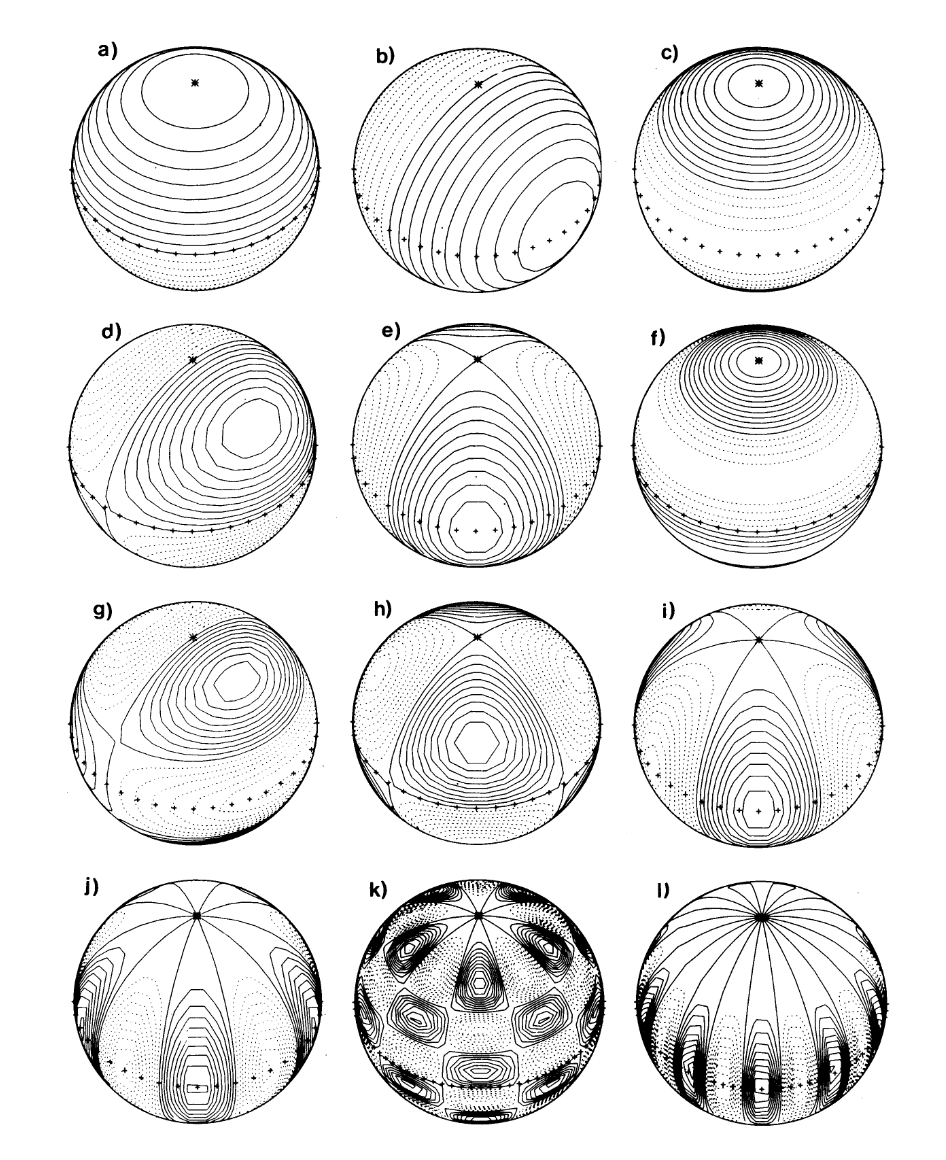
\includegraphics[width=0.9\linewidth]{Imagenes/spherical_harmonics.png}
\caption{Contorno de las partes reales de los armónicos esféricos $Y_m^l$; para simplificar, el factor de fase $(-1)^m$ se ha suprimido. Las líneas de contorno positivas están indicadas por líneas continuas y las negativas por líneas discontinuas. El eje θ = 0 está inclinado en 45º hacia el observador, y se indica con una estrella. El ecuador se muestra como “++++”. Los siguientes casos son ilustrados: a) $l = 1, m = 0$; b) $l = 1, m = 1$; c) $l = 2, m = 0$; d) $l= 2, m = 1$; e) $l = 2, m = 2$; f) $l = 3, m = 0$; g) $l = 3, m = 1$; h) $l = 3, m = 2$; i) $l = 3, m = 3$; j) $l = 5, m = 5$; k) $l = 10, m = 5$; l) $l = 10, m = 10$. Figura tomada de \autocite{ChristensenDalsgaard2019}}
\end{figure}

Al emplear dichos armónicos esféricos como base angular y asumiendo una dependencia temporal armónica de la forma $\exp(-i\omega t)$ (donde $\omega$ es la frecuencia de oscilación propia), podemos escribir las perturbaciones escalares y la componente radial del desplazamiento como:

\begin{align}
\xi_r(r, \theta, \phi, t) &= \sqrt{4\pi}\tilde{\xi}_r(r) Y_l^m(\theta, \phi) \exp(-i\omega t), \\
p'(r, \theta, \phi, t) &= \sqrt{4\pi}\tilde{p}'(r) Y_l^m(\theta, \phi) \exp(-i\omega t),
\end{align}

y de forma análoga para el resto de variables ($\rho', \Phi', \dots$). Las tildes denotan las funciones de amplitud que dependen puramente de la coordenada radial $r$.

Al sustituir estas formas separadas en el sistema de ecuaciones fluido-dinámicas linealizadas derivado en la sección anterior, y recordando que, por la ecuación fundamental que acabamos de resolver, el operador laplaciano horizontal actúa sobre los armónicos esféricos como $\nabla_h^2 Y_l^m = -l(l+1)/r^2 Y_l^m$, podemos dividir todos los términos de las ecuaciones por el factor común $Y_l^m \exp(-i\omega t)$.

Este paso elimina las derivadas angulares y temporales, transformando las ecuaciones en derivadas parciales en un sistema de ecuaciones diferenciales ordinarias (EDOs) unidimensionales para las amplitudes:
\begin{align}
\omega^2 \left[\tilde{\rho}' + \frac{1}{r^2}\frac{d}{dr}(r^2\rho_0\tilde{\xi}_r)\right] &= \frac{l(l+1)}{r^2}(\tilde{p}' + \rho_0\tilde{\Phi}'), \label{eq:1}\\
-\omega^2 \rho_0 \tilde{\xi}_r &= -\frac{d\tilde{p}'}{dr} - \tilde{\rho}'g_0 - \rho_0\frac{d\tilde{\Phi}'}{dr}, \label{eq:2}\\
\frac{1}{r^2}\frac{d}{dr}\left( r^2 \frac{d\tilde{\Phi}'}{dr} \right) - \frac{l(l+1)}{r^2}\tilde{\Phi}' &= 4\pi G \tilde{\rho}', \label{eq:3}
\end{align}

junto con la ecuación de energía adiabática, que se desacopla asumiendo la misma dependencia espacial:
\begin{equation}
(\delta \tilde{p} - \frac{\Gamma_{1,0} p_0}{\rho_0} \delta \tilde{\rho}) = \rho_0(\Gamma_{3,0} - 1)\delta \tilde{q}.
\end{equation}

Como vamos a centrarnos en la aproximación adiabática, el término de ganancia de calor $\delta \tilde{q}$ se anula, simplificando la relación

Es fundamental notar que este sistema depende del grado esférico $l$, pero es totalmente independiente del orden azimutal $m$. Esta degeneración, en la que las frecuencias propias no dependen de $m$, es una consecuencia directa de haber asumido simetría esférica para el estado de equilibrio de la estrella.

\subsection{Oscilaciones Adiabáticas y Condiciones de Contorno}

Para oscilaciones adiabáticas, tenemos que $\delta q = 0$, y podemos reescribir la ecuación de energía como: 

\begin{equation}
    \rho' = \frac{\rho}{\Gamma_1 p} p' + \rho \xi_r \left(\frac{1}{\Gamma_1 p}\frac{dp}{dr} - \frac{1}{\rho}\frac{d\rho}{dr} \right),
\end{equation}

donde hemos suprimido la tilde en las funciones de amplitud y el ``0'' en las cantidades de equilibrio para simplificar la notación. . Este cambio no debería causar confusión.

Podemos utilizar esta ecuación para eliminar $\rho'$ de las ecuaciones \eqref{eq:1} - \eqref{eq:3} y reescribirlas de la siguiente manera:

La ecuación \eqref{eq:1} se convierte en:

\begin{equation}
    \frac{d\xi_r}{dr} = -\left(\frac{2}{r}+\frac{1}{\Gamma_1 p}\frac{dp}{dr}\right)\xi_r + \frac{1}{\rho c^2}\left(\frac{S_l^2}{\omega^2}-1\right) p' + \frac{l(l+1)}{\omega^2 r^2} \Phi',
\end{equation}

donde se introduce la frecuencia acústica característica $S_l$ (o de Lamb) como:
$$S_l^2 = \frac{l(l+1)c^2}{r^2}=k_h^2c^2$$

La ecuación \eqref{eq:2} nos da:
\begin{equation}
    \frac{dp'}{dr} = \rho(\omega^2 - N^2)\xi_r + \frac{1}{\Gamma_1 p}\frac{dp}{dr}p' - \rho \frac{d\Phi'}{dr},
\end{equation}
siendo N la frecuencia de flotabilidad (o de Brunt-Väisälä), dada por:
$$N = g\left(\frac{1}{\Gamma_1 p}\frac{dp}{dr} - \frac{1}{\rho}\frac{d\rho}{dr} \right).$$

Finalmente, la ecuación \eqref{eq:3} se puede escribir como:

\begin{equation}
    \frac{1}{r^2}\frac{d}{dr} \left(r^2\frac{d\Phi'}{dr}\right) = 4\pi G\left( \frac{p'}{c^2} + \frac{\rho \xi_r}{g} N^2\right) + \frac{l(l+1)}{r^2} \Phi'.
\end{equation}

El sistema que acabamos de obtener es un sistema de ecuaciones diferenciales ordinarias de cuarto orden con las variables dependientes $\xi_r$, $\Phi'$, $p'$ y $d\Phi'/dr$. Para que dicho problema esté matemáticamente bien planteado, al tratar con un sistema diferencial de cuarto orden, es imperativo establecer cuatro condiciones de contorno físicas, las cuales pueden encontrarse en la literatura con más detalle:

\begin{itemize}
\item \textbf{En el centro ($r=0$):} Este punto representa una singularidad regular en las ecuaciones. Como es habitual en la teoría de ecuaciones diferenciales, el sistema admite tanto soluciones regulares como singulares en este punto, por lo que dos de las condiciones sirven para seleccionar únicamente las soluciones regulares. Expandiendo las ecuaciones cerca de $r=0$, se demuestra que el desplazamiento $\xi_r$ se comporta como $r^{l-1}$, mientras que $p'$ y $\Phi'$ se comportan como $r^l$. En el caso particular de las oscilaciones radiales, el coeficiente del término de orden principal de $\xi_r$ se anula, de manera que $\xi_r$ es proporcional a $r$. De hecho, por consideraciones geométricas, es evidente que para oscilaciones con simetría esférica el desplazamiento debe anularse en el centro. Además, a partir de estas expansiones, se obtiene que para $l>0$, las soluciones cerca del centro cumplen la relación $\xi_r \simeq l\xi_h$ cuando $r \rightarrow 0$. 

\item \textbf{En la superficie ($r=R$):} Asumiendo que se asigna a la estrella un límite definido en $r=R$, es físicamente razonable suponer que dicha superficie exterior está libre, de modo que no actúan fuerzas sobre ella y el sistema se puede considerar como un sistema aislado. Esto equivale a exigir que la presión sea constante en la superficie perturbada. Por lo tanto, como condición de contorno en la superficie se toma que la perturbación de presión lagrangiana se anule, es decir, $\delta p = p' + \xi_r \frac{dp}{dr} = 0$ en $r=R$. 
Por último, se exige la continuidad de la perturbación del potencial gravitatorio ($\Phi'$) y de su primera derivada en el radio de la superficie ($r=R$). Dado que fuera de la estrella la perturbación de densidad se anula, la ecuación de Poisson puede resolverse de forma analítica. La solución que decae y se anula en el infinito es $\Phi' = A r^{-l-1}$. Como consecuencia, $\Phi'$ debe satisfacer la siguiente condición matemática empalmando con el vacío exterior:
\begin{equation}
    \frac{d\Phi'}{dr} + \frac{l+1}{r}\Phi' = 0 \quad \text{en } r=R.
\end{equation} 
Como información adicional derivada de la condición de la presión, se puede aproximar que la proporción entre el desplazamiento horizontal y radial en la superficie depende únicamente de la frecuencia adimensional ($\sigma$), dada por $\frac{\xi_h(R)}{\xi_r(R)} \approx \sigma^{-2}$.
\end{itemize}
\section{Naturaleza y Clasificación de los Modos de Oscilación}

\subsection{La Aproximación de Cowling} 

Para analizar analíticamente las oscilaciones, a menudo se asume que la perturbación del potencial gravitatorio es despreciable $(\Phi' \approx 0)$. Esta simplificación es válida para grados $l$ grandes o cuando el orden radial $|n|$ es alto. Bajo esta aproximación, el sistema de cuarto orden se reduce a dos ecuaciones diferenciales de primer orden:
\begin{align}
 \frac{d\xi_r}{dr} &= -\left(\frac{2}{r} - \frac{1}{\Gamma_1 H_p}\right)\xi_r + \frac{1}{\rho c^2}\left(\frac{S_l^2}{\omega^2} - 1\right)p' \\
 \frac{dp'}{dr} &= \rho(\omega^2 - N^2)\xi_r - \frac{1}{\Gamma_1 H_p}p',
\end{align}

donde $H_p = -(d \ln p / dr)^{-1}$ es la escala de altura de presión.

\subsection{Frecuencias Características y Atrapamiento} 
Para modos de alto orden radial, las autofunciones varían mucho más rápido que las cantidades de equilibrio. Despreciando las derivadas de estas últimas, el sistema anterior se combina en una única ecuación diferencial de segundo orden que describe el comportamiento local de las ondas: 
$$\frac{d^2\xi_r}{dr^2} = -K(r)\xi_r,$$  

donde la función K(r) viene dada por:
\begin{equation}
    K(r) = \frac{\omega^2}{c^2} \left( \frac{N^2}{\omega^2} - 1 \right) \left( \frac{S_l^2}{\omega^2} - 1 \right)
\end{equation}

La propagación depende de las dos frecuencias características: la frecuencia acústica $(S_l)$ y la de flotabilidad $(N)$. La solución es oscilatoria $(\xi_r \sim \cos(\int K^{1/2} dr + \phi))$ en las regiones de ``atrapamiento'' donde $K(r) > 0$. Fuera de estas regiones $(K(r) < 0)$, la solución decae exponencialmente. Los límites de atrapamiento se sitúan en los puntos de retorno geométricos, donde $K(r) = 0.$

\begin{figure}[htbp]
    \centering
    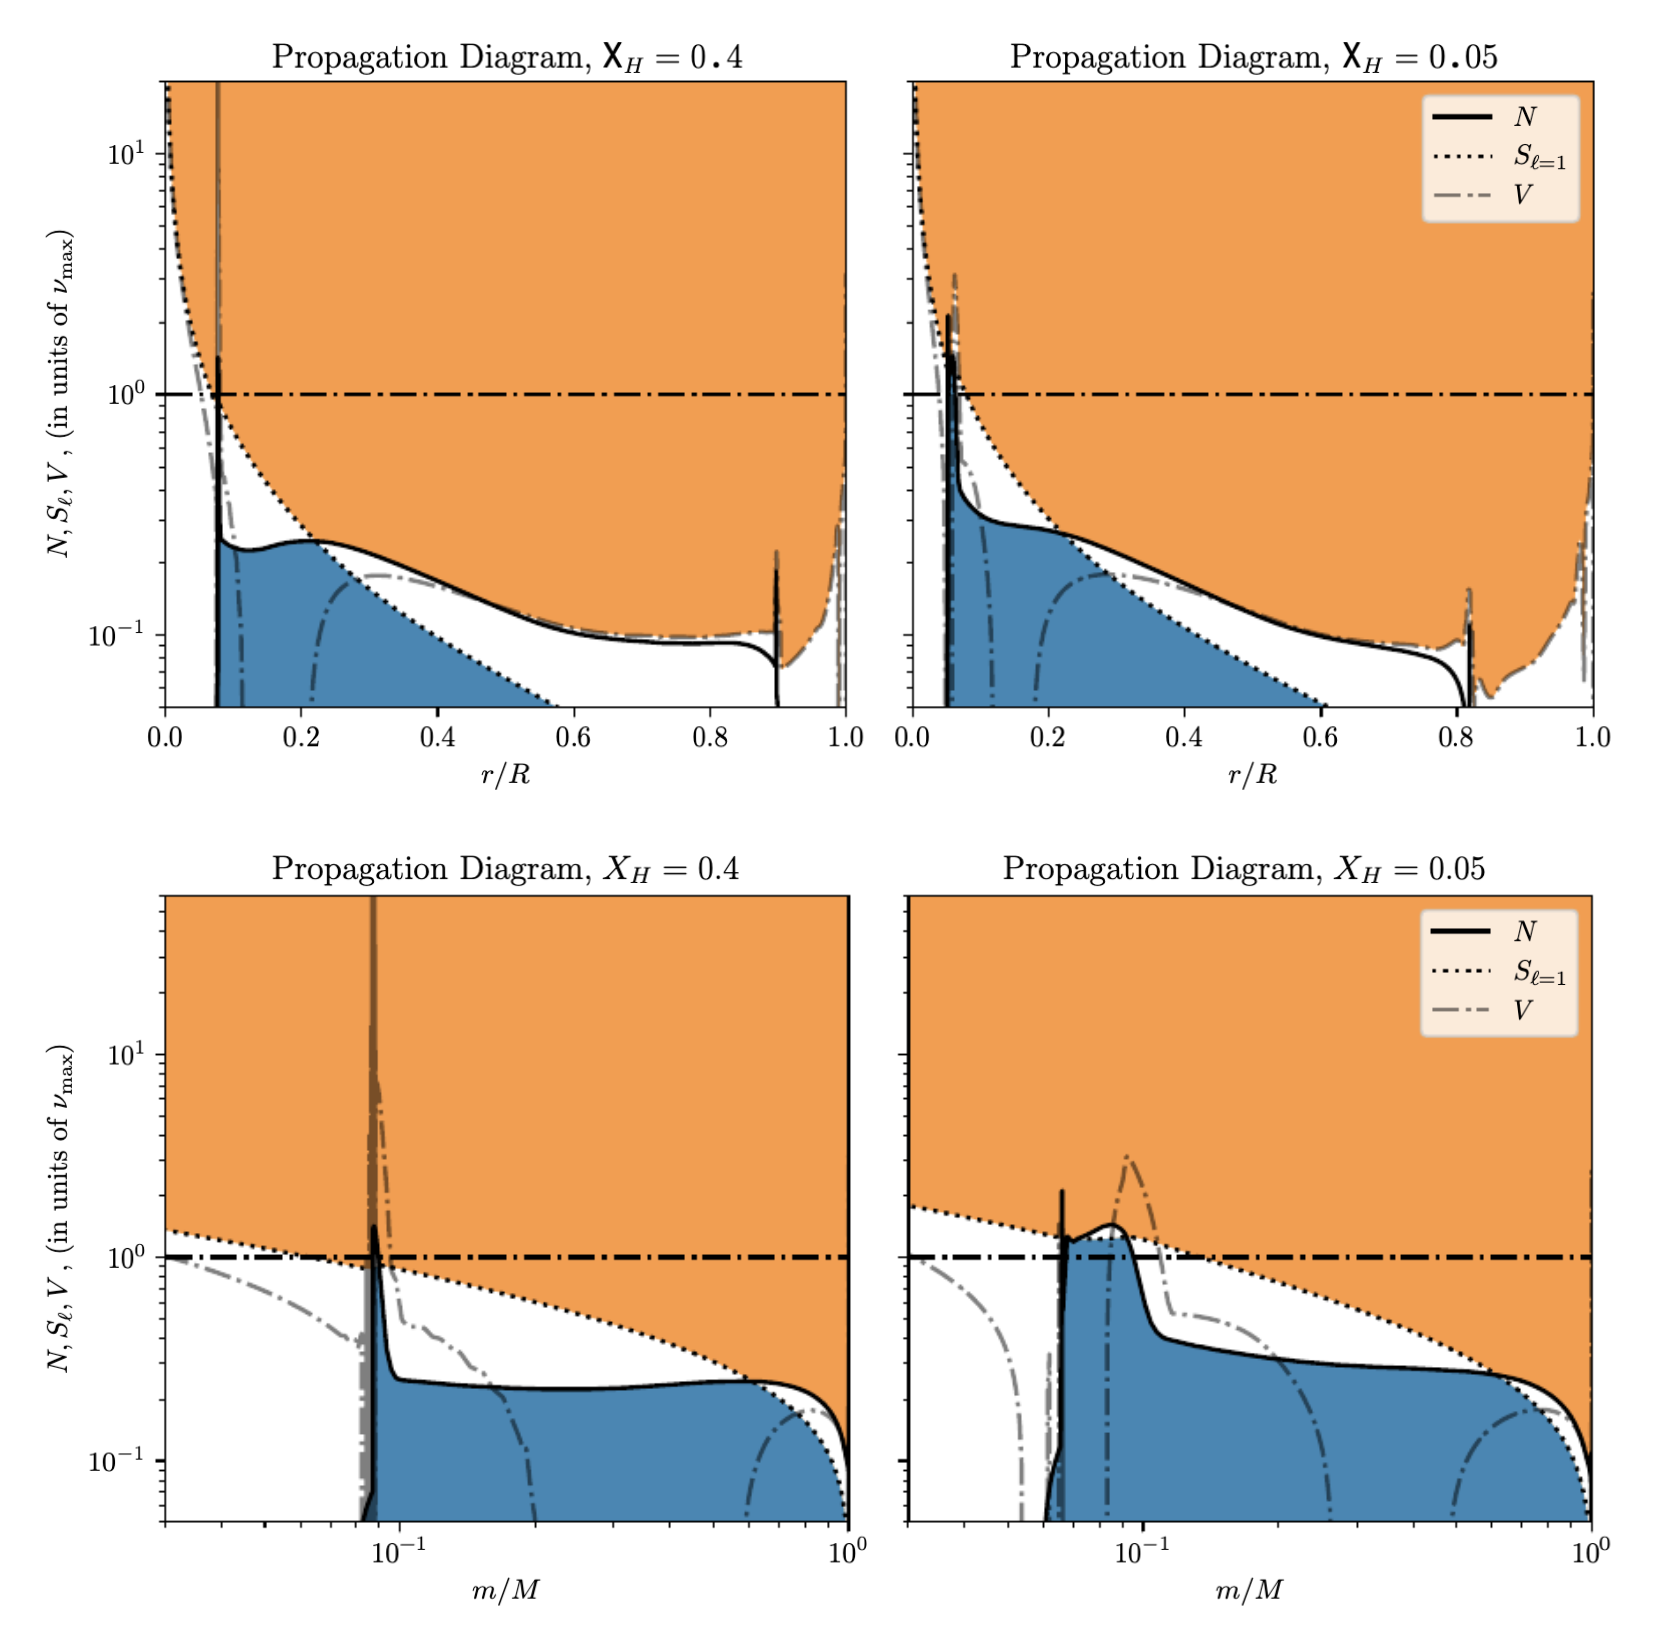
\includegraphics[width=0.9\textwidth]{Imagenes/prop_diagrams.png}
    \caption{Diagrama de propagación para un modelo de $1.4 M_\odot$ con $X_H=0.4$ (línea vertical gris punteada más a la izquierda en Fig. 1) que muestra, en unidades de $\nu_{\text{max}}$, las frecuencias de flotabilidad ($N$), la frecuencia de Lamb ($S_{l=1}$) y el potencial acústico, $V$, que es una frecuencia característica que describe la propagación de los modos radiales de una estrella. La región naranja del diagrama de propagación representa las regiones donde se pueden propagar modos p, mientras que las regiones azules representan las regiones de propagación de modos g. En las capas exteriores de la estrella, la frecuencia mínima a la cual se pueden propagar los modos p está determinada por la frecuencia crítica ($\nu_{\text{crit}}$ imita $V$ cerca de la superficie del modelo) en las capas exteriores. \textbf{Panel superior derecho:} El mismo panel que el anterior pero para el modelo de $1.4 M_\odot$ más tarde en su evolución (línea gris punteada a la derecha en Fig. 1, $X_H=0.05$). \textbf{Paneles inferiores:} Diagrama de propagación para los mismos dos modelos que los superiores, pero el eje x muestra la coordenada relativa de masa en escala logarítmica para mostrar las características cercanas al núcleo en mayor detalle. El potencial acústico, $V$, muestra un pico localizado y agudo en la parte cercana al núcleo.}
    \label{fig:prop_diagrams}
\end{figure}

\subsection{Modos de Presión (p-modes)} 

Corresponden a la rama de altas frecuencias donde $\omega \gg N$. En este límite, la función $K(r)$ se aproxima a:

$$K(r) \simeq \frac{1}{c^2}(\omega^2 - S_l^2)$$

La dinámica está dominada por la velocidad del sonido c (ondas acústicas). La condición del punto de retorno interno $(r_t)$, obtenida al igualar $S_l(r_t) = \omega$, es:

$$\frac{c^2(r_t)}{r_t^2} = \frac{\omega^2}{l(l+1)}$$  

A partir de la relación de dispersión para ondas sonoras planas, el número de onda radial al cuadrado se identifica de forma natural con K:

$$k_r^2 = \frac{1}{c^2}(\omega^2 - S_l^2)$$

En los modos p, la frecuencia de oscilación aumenta con el orden del modo.

\subsection{Modos de Gravedad (g-modes)} 
Corresponden a la rama de bajas frecuencias, encontradas en el interior profundo estelar, donde $\omega^2 \ll S_l^2$. La aproximación para K(r) se convierte en:

$$ K(r) \simeq \frac{1}{\omega^2}(N^2 - \omega^2) \frac{l(l+1)}{r^2} $$

Aquí, la dinámica está controlada por la variación de la frecuencia de flotabilidad $N$, siendo la gravedad la fuerza restauradora sobre las perturbaciones de densidad. Los puntos de retorno vienen dados por la condición $N = \omega$. En congruencia con las ondas de gravedad estacionarias, su número de onda radial es:

$$k_r^2 = \frac{l(l+1)}{r^2}\left(\frac{N^2}{\omega^2} - 1\right)$$

A diferencia de los p-modes, en los modos g el orden aumenta a medida que disminuye $\omega$, y su frecuencia máxima está limitada estrictamente por el valor máximo de $N$ en el interior de la estrella.

\begin{figure}[htbp]
    \centering
    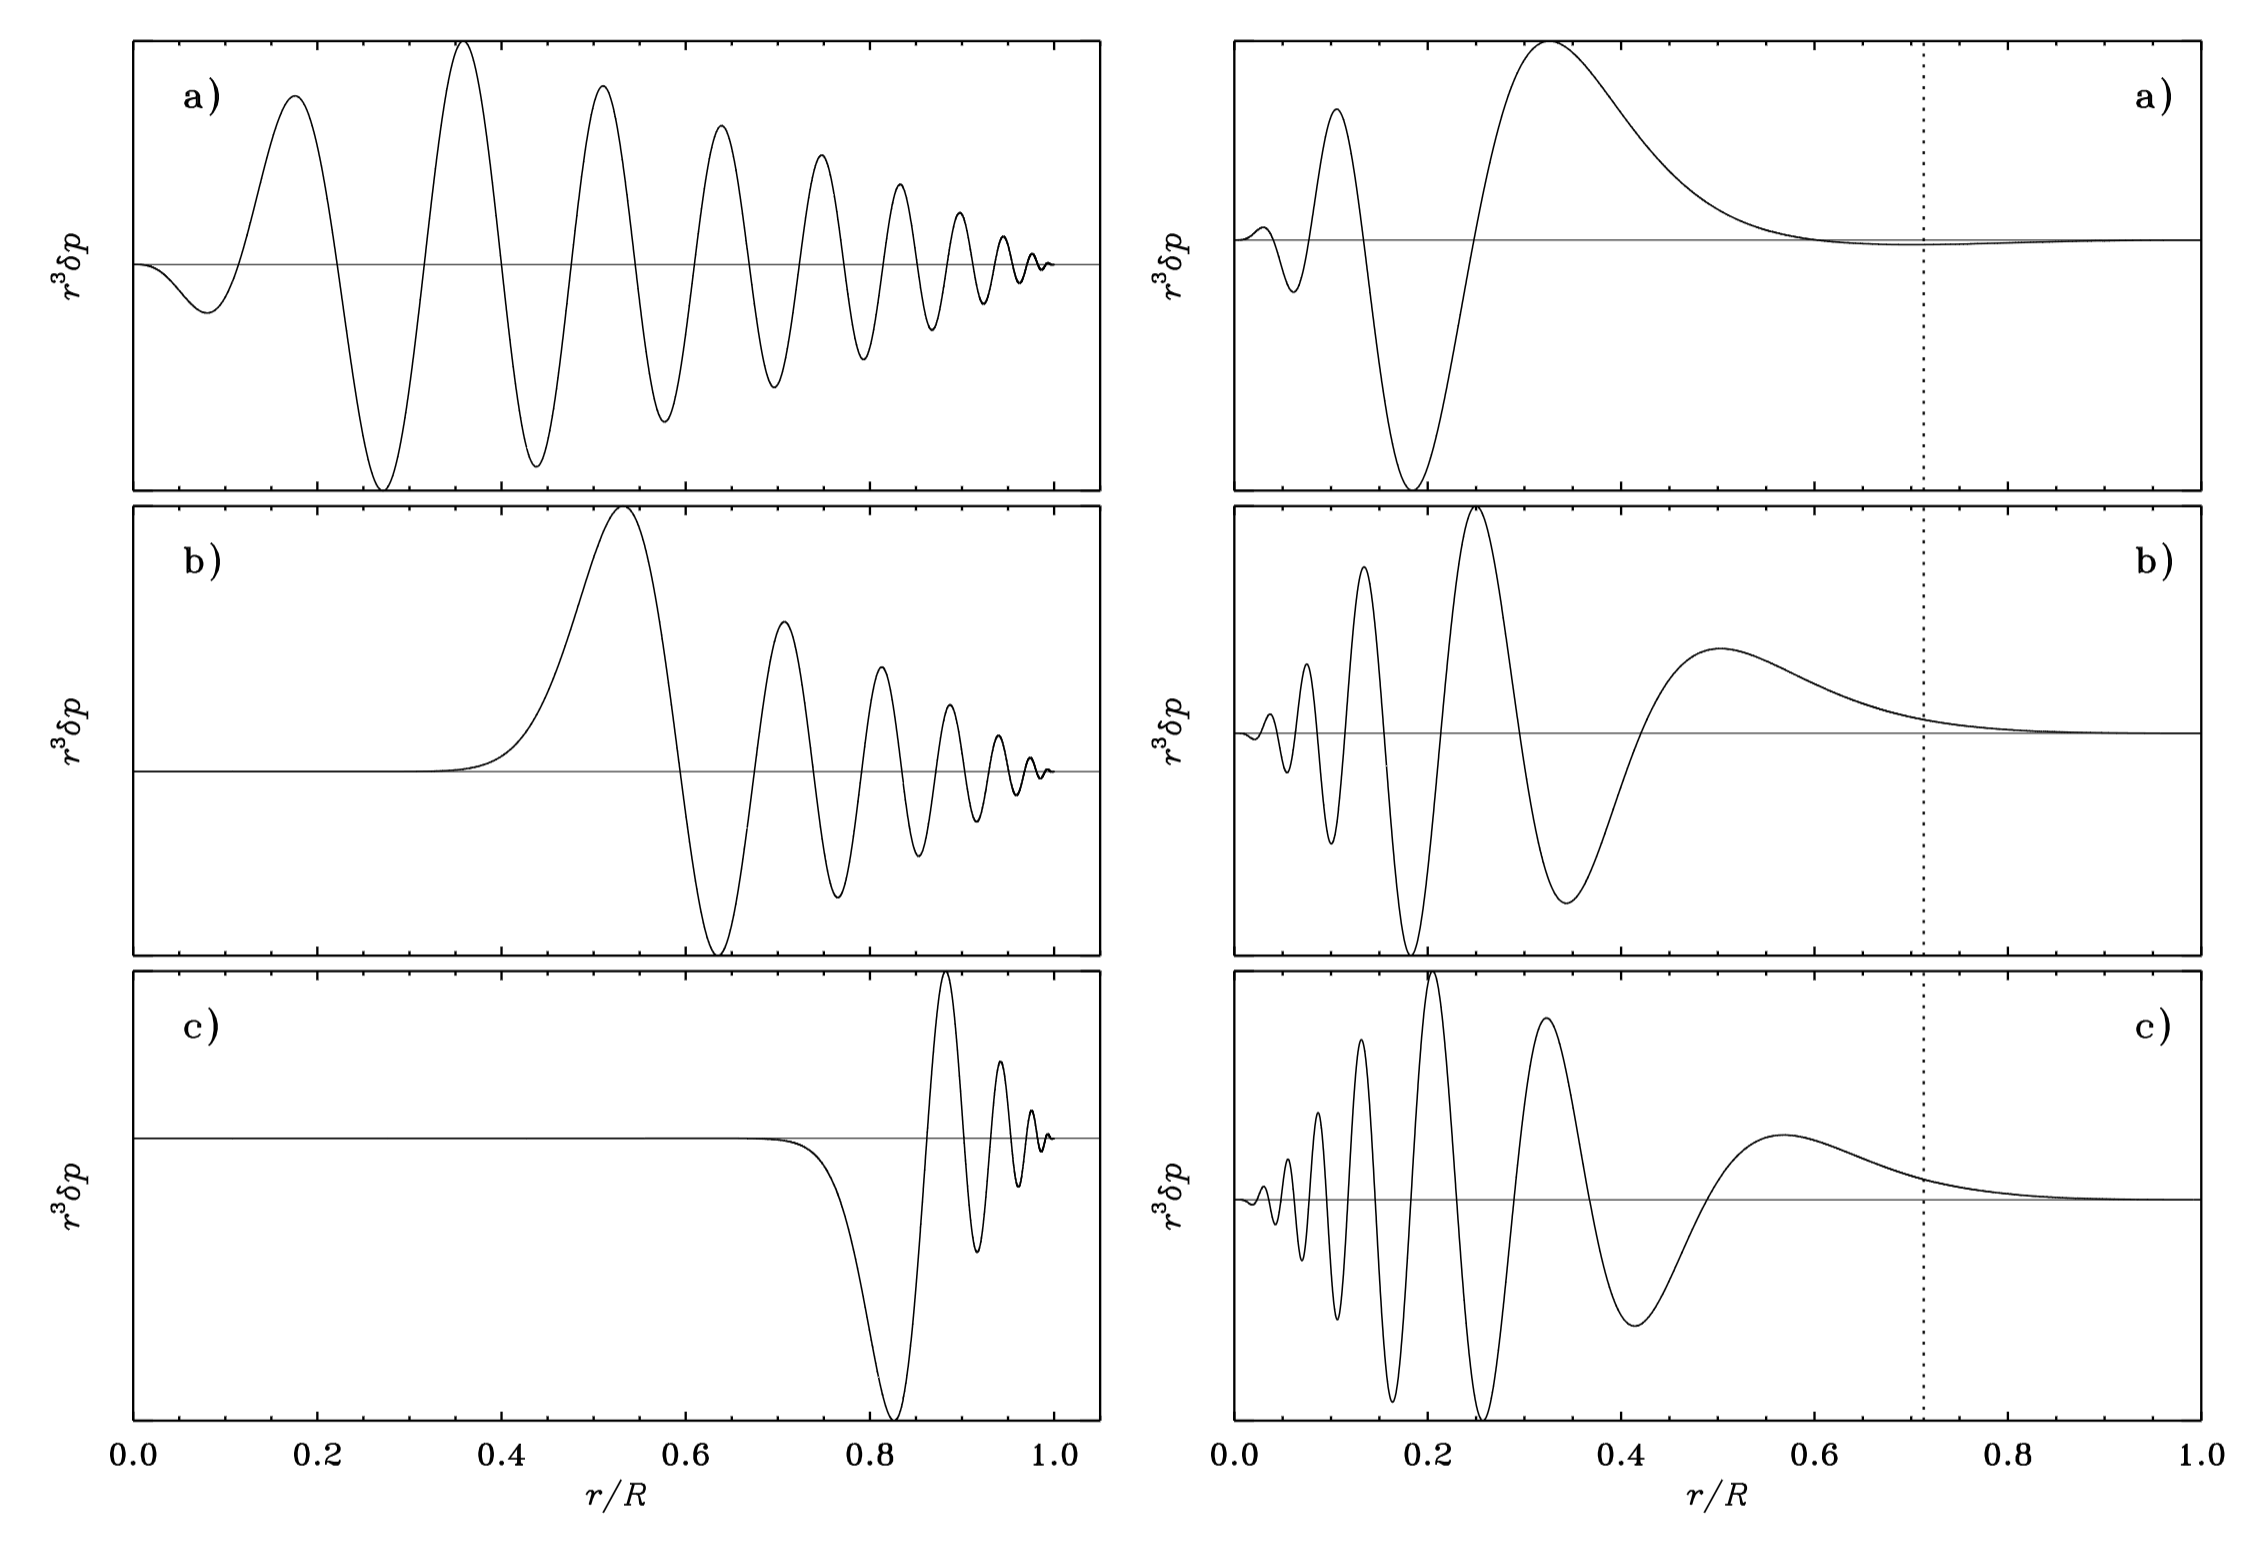
\includegraphics[width=\textwidth]{Imagenes/eigenfunctions.png}
    \caption{Autofunciones normalizadas para un modelo del Sol, en función del radio fraccional. La autofunción elegida, $r^3\delta p$, tiene las dimensiones de energía y está normalizada a su valor máximo. Izquierda: Resultados para 3 modos p: a) ($l = 0, n = 21, \nu = 3038.0\mu$Hz), b) ($l = 20, n = 14, \nu = 2939.2\mu$Hz), y c) ($l = 60, n = 9, \nu = 3043.2\mu$Hz). Derecha: Resultados para 3 modos g: a) ($l = 1, n = -5, \nu = 109.2\mu$Hz), b) ($l = 2, n = -10, \nu = 102.6\mu$Hz), y c) ($l = 3, n = -14, \nu = 104.1\mu$Hz). La línea punteada marca la base de la envoltura convectiva. Imagen tomada de \autocite{Cunha2017}.}
    \label{fig:eigenfunctions_pg_modes}
\end{figure}

\chapter{Creando Blue Stragglers}

En este capítulo expondré las técnicas utilizadas para simular la formación de Blue Stragglers utilizando MESA.

\section{MESA}
MESA (\textit{Modules for Experiments in Stellar Astrophysics}) es un entorno numérico de código abierto diseñado para simular la estructura y evolución estelar en una dimensión (1D) \citep{paxton2011, paxton2013, paxton2015, paxton2018, paxton2019, jermyn2023}. Gracias a su arquitectura modular, alta paralelización y un solucionador completamente implícito, MESA permite modelar una amplia gama de configuraciones estelares y escenarios evolutivos dinámicos o estacionarios.

A diferencia de los códigos tradicionales de evolución estelar, MESA está escrito en Fortran moderno y se caracteriza por una separación estricta entre la física del interior estelar y la maquinaria numérica del solver. Su desarrollo activo por parte de una amplia comunidad científica asegura la continua actualización de las bases físicas y la optimización de los algoritmos numéricos.

\subsection{Funcionamiento de MESA y Ecuaciones Base}
El núcleo de MESA resuelve simultáneamente, en un esquema de diferencias finitas completamente implícito unidimensional, el sistema de ecuaciones diferenciales en derivadas parciales acopladas que rige la estructura y evolución estelar en coordenadas lagrangianas de masa $m$:

\begin{enumerate}
    \item \textbf{Ecuación de conservación de la masa:} Relaciona el radio del elemento de fluido estelar con su densidad de masa local $\rho$:
    \begin{equation}
        \frac{\partial r}{\partial m} = \frac{1}{4\pi r^2 \rho}
    \end{equation}

    \item \textbf{Ecuación de equilibrio hidrostático:} Describe el balance de fuerzas mecánicas, incluyendo el término de aceleración inercial fundamental para fases de evolución rápida:
    \begin{equation}
        \frac{\partial P}{\partial m} = -\frac{G m}{4\pi r^4} - \frac{1}{4\pi r^2}\frac{\partial^2 r}{\partial t^2}
    \end{equation}
    donde $P$ es la presión local y $G$ es la constante de gravitación universal.

    \item \textbf{Ecuación de conservación de la energía:} Determina la luminosidad $L$ en función de la generación de energía interna:
    \begin{equation}
        \frac{\partial L}{\partial m} = \epsilon_{\text{nuc}} - \epsilon_\nu + \epsilon_{\text{grav}}
    \end{equation}
    siendo $\epsilon_{\text{nuc}}$ la tasa de generación de energía nuclear por unidad de masa, $\epsilon_\nu$ las pérdidas por neutrinos y $\epsilon_{\text{grav}}$ el término de energía térmica o gravitatoria definido como:
    \begin{equation}
        \epsilon_{\text{grav}} \equiv -T \frac{\partial s}{\partial t}
    \end{equation}
    donde $T$ es la temperatura local y $s$ es la entropía específica del gas.

    \item \textbf{Ecuación de transporte de energía:} Determina el gradiente térmico necesario para transportar la energía producida:
    \begin{equation}
        \frac{\partial T}{\partial m} = -\frac{G m T}{4\pi r^4 P} \nabla
    \end{equation}
    donde el gradiente de temperatura local $\nabla \equiv \frac{\partial \ln T}{\partial \ln P}$ se define según el mecanismo de transporte dominante:
    \begin{equation}
        \nabla = 
        \begin{cases} 
          \nabla_{\text{rad}} = \frac{3 \kappa L P}{16 \pi G m a c T^4} & \text{en regiones radiativas (estable),} \\
          \nabla_{\text{conv}} & \text{en regiones convectivas.}
        \end{cases}
    \end{equation}
    Aquí, $\kappa$ representa la opacidad del gas, $a$ la constante de densidad de radiación y $c$ la velocidad de la luz. En regiones convectivas inestables, MESA calcula $\nabla_{\text{conv}}$ aplicando la teoría de la longitud de mezcla estándar (\textit{Mixing Length Theory}, MLT).
\end{enumerate}

El solver de MESA resuelve estas ecuaciones simultáneamente aplicando un método de Newton-Raphson de múltiples variables. Utiliza un esquema de discretización espacial adaptativa (malla móvil) que refina automáticamente el número y la distribución de las celdas en zonas con fuertes gradientes físicos (como límites de zonas convectivas, frentes de combustión nuclear o la atmósfera estelar). El paso de tiempo también se ajusta dinámicamente según la convergencia y la tasa de cambio de las variables termodinámicas de la estrella.

\subsubsection{Módulos y Física Integrada}
La modularidad de MESA radica en que las diferentes propiedades físicas se calculan a través de módulos independientes e intercambiables que se comunican con el solver principal. Los módulos clave implicados en nuestras simulaciones son:

\begin{itemize}
    \item \texttt{mesa/star}: El resolvedor central que orquesta la integración temporal y espacial.
    \item \texttt{mesa/eos}: La ecuación de estado (EOS), que calcula la presión, entropía y demás variables termodinámicas en función de la densidad, temperatura y composición química. Utiliza una combinación de tablas (OPAL, SCVH, HELM y PC) adaptada a cada rango de densidad y temperatura.
    \item \texttt{mesa/kap}: Módulo de opacidades. En nuestras simulaciones se activaron las opacidades avanzadas de tipo 2 (\texttt{use\_Type2\_opacities = .true.}), con una metalicidad base de $Z_{\text{base}} = 0.02$, permitiendo evaluar los efectos térmicos de las variaciones locales de carbono, nitrógeno y oxígeno en la envoltura estelar debido al material transferido.
    \item \texttt{mesa/net}: La red de reacciones nucleares que determina la nucleosíntesis y la generación de energía nuclear $\epsilon_{\text{nuc}}$.
    \item \texttt{mesa/binary}: Módulo de evolución binaria que acopla dinámicamente dos modelos estelares independientes a través de interacciones orbitales y transferencia de masa.
\end{itemize}

Para configurar estos módulos, los usuarios emplean archivos de configuración con formato de lista de variables (\textit{namelist}) de Fortran, denominados colectivamente \textit{inlists} (por ejemplo, \texttt{inlist\_project}, \texttt{inlist\_pgstar}). Esto permite modificar las condiciones físicas y los parámetros del solver sin necesidad de compilar el código fuente general del entorno.

\subsection{MESA y la formación de Blue Stragglers}
La formación de Blue Stragglers mediante la vía de transferencia de masa en sistemas binarios se modela a través del módulo \texttt{mesa/binary}. Este módulo calcula de manera simultánea la evolución de ambas estrellas (donante y acretora) y los parámetros orbitales como la separación angular y el período orbital.

\subsubsection{Modelado de la Transferencia de Masa por Desbordamiento del Lóbulo de Roche}
El inicio de la transferencia de masa se define cuando el radio de la estrella donante supera el radio equivalente de su lóbulo de Roche ($R_1 \geq R_{\text{L},1}$), aproximado mediante la expresión de Eggleton \citep{eggleton1983}:
\begin{equation}
    R_{\text{L},1} = a \frac{0.49 q^{2/3}}{0.6 q^{2/3} + \ln(1 + q^{1/3})}
\end{equation}
donde $a$ es la separación orbital del sistema y $q = M_1/M_2$ es la relación de masas. El ritmo de pérdida de masa de la estrella donante se calcula utilizando la formulación implícita de Ritter \citep{ritter1988, kolbritter1990}, que evalúa el desbordamiento basándose en la escala de altura de presión en las capas superficiales de la atmósfera estelar.

Nuestra simulación modela la formación de una Blue Straggler a partir de un sistema binario inicial con las siguientes características:
\begin{itemize}
    \item \textbf{Estrella donante ($M_1$):} Masa inicial de $2.0\,M_\odot$, configurada con el archivo \texttt{inlist1}.
    \item \textbf{Estrella acretora ($M_2$):} Masa inicial de $1.0\,M_\odot$, configurada con el archivo \texttt{inlist2}.
    \item \textbf{Período orbital inicial:} $4.0$ días (\texttt{initial\_period\_in\_days = 4d0}).
\end{itemize}

El proceso de transferencia de masa se modela bajo una hipótesis de \textbf{transferencia de masa no conservativa}, parametrizada mediante el coeficiente $\beta = 0.5$ (\texttt{mass\_transfer\_beta = 0.5d0}). Esto significa que el 50\% de la masa transferida por la estrella donante es retenida por la acretora, mientras que el otro 50\% es expulsado del vecindario de la estrella acretora. Esta materia perdida abandona el sistema portando el momento angular específico de la órbita de la acretora, lo cual tiene un efecto estabilizador en la evolución orbital al ensanchar el semieje mayor.

\subsubsection{Estabilidad Numérica del Acretor y Ajustes del Solver}
La adición acelerada de material caliente sobre la estrella de $1.0\,M_\odot$ introduce perturbaciones térmicas y mecánicas drásticas en sus capas más externas. Esto provoca una expansión violenta de su envoltura convectiva y puede llevar a una caída de la luminosidad superficial por debajo de cero, deteniendo la convergencia numérica. Para mitigar esto, se aplican límites estrictos sobre la tasa de transferencia de masa implícita y explícita admisible por paso de tiempo a un valor máximo de $10^{-4}\,M_\odot/\text{año}$ (\texttt{max\_implicit\_abs\_mdot = 1d-4}).

Desde el punto de vista físico, la envoltura externa del acretor es altamente superadiabática y está dominada por la presión de radiación. Para estabilizar este frente numéricamente, se activa el esquema \texttt{MLT++} en MESA (\texttt{okay\_to\_reduce\_gradT\_excess = .true.}). Este método reduce artificialmente la superadición del gradiente de temperatura en regiones donde la eficiencia del transporte convectivo es extremadamente baja pero la radiación ejerce una presión dominante, facilitando la convergencia sin alterar la estructura profunda de la estrella.

Adicionalmente, se ajusta la tolerancia del resolvedor aumentando el coeficiente de resolución espacial superficial (\texttt{mesh\_delta\_coeff = 0.5}) para refinar el mallado del perfil y se relaja ligeramente el residuo máximo admisible a $10^{-3}$ (\texttt{gold\_tol\_max\_residual3 = 1d-3}) para evitar fallos del solver debidos al ruido numérico inducido por la acreción rápida. El control de paso de tiempo durante la fase de desbordamiento (RLOF) se restringe rígidamente utilizando los parámetros adimensionales \texttt{fm = 0.001}, \texttt{fr = 0.01} y \texttt{fj = 0.01} (que limitan los cambios fraccionales de masa, radio y momento angular en cada iteración).

\subsubsection{Acoplamiento con GYRE para Análisis Astrosismológico}
Una vez finalizada la fase de transferencia de masa, el modelo rejuvenecido resultante adquiere una masa final de $1.82136\,M_\odot$ y una estructura química interna alterada (con un núcleo enriquecido en helio y una envoltura rica en hidrógeno depositado). Esta Blue Straggler recién formada se evoluciona en una configuración de estrella aislada (\texttt{evolve\_created\_blue\_straggler}) a partir del modelo binario de salida, extendiendo la simulación hasta que la fracción de masa de hidrógeno central cae por debajo de $10^{-3}$ (\texttt{xa\_central\_lower\_limit(1) = 1d-3}), lo que define la TAMS (\textit{Terminal Age Main Sequence}).

Para poder comparar las firmas espectrales de este modelo con estrellas normales, se genera de manera paralela una rejilla de modelos de control unidimensionales estándar utilizando el script \texttt{create\_mass\_grid.py} en el directorio \texttt{mass\_grid}. Esta rejilla abarca masas desde $1.75\,M_\odot$ hasta $1.89\,M_\odot$ con un incremento de $0.01\,M_\odot$, evolucionándose bajo las mismas condiciones físicas físicas base ($Z = 0.02$, opacidades tipo 2, $\text{X}_{\text{c}} \leq 10^{-3}$).

Durante toda la evolución del modelo rejuvenecido y de la rejilla de control, MESA vuelca perfiles de estructura estelar en formato compatible con el código de oscilaciones estelares **GYRE** \citep{townsend2013} (\texttt{pulse\_data\_format = 'GYRE'}). 

El análisis de oscilaciones estelares se automatiza mediante el script de shell \texttt{run\_gyre\_all.sh}, el cual realiza los siguientes pasos para cada perfil estructural guardado:
\begin{enumerate}
    \item Genera dinámicamente un archivo de parámetros \texttt{gyre.in} reemplazando la ruta del perfil de entrada y especificando los archivos de salida HDF5 correspondientes para el resumen de modos (\texttt{summary.h5}) y las funciones propias detalladas (\texttt{detail.l\%l.n\%n.h5}).
    \item Resuelve las ecuaciones lineales de pulsación no adiabáticas o adiabáticas para los grados armónicos esféricos $l = 0$ (modos radiales), $l = 1$ (modos dipolares) y $l = 2$ (modos cuadrupolares) utilizando un esquema de colocación de cuarto orden (\texttt{COLLOC\_GL4}).
    \item Realiza un barrido lineal en frecuencia entre $0.1$ y $20$ ciclos por día (\texttt{freq\_min = 0.1}, \texttt{freq\_max = 20}) con $3000$ puntos para identificar los autovalores de frecuencia y las amplitudes de los desplazamientos radiales ($\xi_r$) y horizontales ($\xi_h$).
\end{enumerate}

Este acoplamiento numérico entre MESA y GYRE permite discernir las sutiles diferencias en la frecuencia acústica característica (frecuencia de Lamb $S_l$) y de flotabilidad (Brunt-Väisälä $N$) entre la Blue Straggler y las estrellas ordinarias de la secuencia principal de idéntica masa, ofreciendo un método directo para verificar los modelos de rejuvenecimiento frente a observaciones astrosismológicas reales (como las proyectadas en la misión espacial HAYDN).


%\input{Capítulos/Resultados}
%\chapter{Conclusiones}

En este trabajo se ha llevado a cabo un trabajo teórico y computacional para evaluar la capacidad de la astrosismología de diferenciar dos historias evolutivas distintas que producen estrellas en idéntica posición del diagrama HR: la hipótesis aislada y la hipótesis de transferencia de masa binaria en el contexto de la formación de Blue Stragglers. Para ello se ha combinado el uso del código de evolución estelar MESA con el de oscilación, GYRE. Con los resultados obtenidos, se han calculado las diferencias en gran separación, pequeña separación y frecuencias individuales que cabría esperar entre una Blue Straggler y una estrella ``simple''. A continuación, se resumen los resultados y las limitaciones del estudio.

\section{Resultados Principales}

\subsection{Simulación de la Blue Straggler y estrellas de referencia}

Se ha simulado la creación de una Blue Straggler en la etapa evolutiva de secuencia principal temprana (Caso A) a través de la transferencia de masa, empleando para ello el módulo \texttt{binary} de MESA. El sistema binario se componía de una estrella donante de $2.0~M_\odot$ y una acretora de $1.0~M_\odot$, con un periodo orbital de 4 días. La transferencia de masa comienza alrededor de $t_0 = 909.3~\text{Myr}$ y da lugar a una estrella rejuvenecida de $1.82136~M_\odot$ con una estructura interior claramente distinta a la de una estrella de masa similar con evolución aislada: un núcleo enriquecido con hidrógeno nuevo y helio más diluido (Figura \ref{fig:evolution_graphs}), y un perfil de composición química alterado en sus capas intermedias. Esta estructura interna modificada es la señal que la astrosismología debe detectar.

Además, se ha empleado el repositorio \texttt{wsssss} para simular una cuadrícula de estrellas de masa similar a la de la Blue Straggler, con el fin de emplearlas para comparar sus frecuencias de oscilación, y poder determinar si la astrosismología puede diferenciar ambos escenarios evolutivos.

\subsection{Diferencias en la Gran Separación}

Las grandes separaciones ($\Delta\nu$) de la Blue Straggler y de las estrellas de referencia se han calculado de forma similar a como se haría en un estudio observacional (calculando el espectro de frecuencias de la estrella y obteniendo la diferencia de frecuencia entre modos de órdenes radiales consecutivos). En este caso, dado que se disponía de las frecuencias calculadas directamente por GYRE, no ha sido necesario calcular dicho espectro de frecuencias, y se han empleado directamente estas frecuencias.

Se han comparado las diferencias en grandes separaciones para 7 puntos significativos de la evolución de la Blue Straggler (representados en la Figura \ref{fig:global_hr_diagram}), abarcando desde $H_c \approx 69.7\%$ hasta $H_c \approx 0.1\%$. Las diferencias más notables se identifican en los modos no radiales, especialmente para $l=2$, con valores máximos que alcanzan $|\Delta(\Delta\nu)|_{\max}^{l=2} \approx 2.491\,\text{ciclos\,día}^{-1}$ en las etapas más tardías de la secuencia principal. Además se ha observado que las diferencias para $l=0$ son comparativamente menores, llegando el cociente $r = |\Delta(\Delta\nu)|_{\max}^{l=2} / |\Delta(\Delta\nu)|_{\max}^{l=0}$ a valores como $88.5$ para el Par 7. Todo esto confirma que los modos cuadrupolares son significativamente más sensibles a las diferencias internas que existen entre una BSS y una estrella simple.

\subsection{Diferencias en Frecuencias Individuales}

Al comparar las frecuencias individuales para estos mismos 7 puntos, se observa que en los modos radiales ($l=0$) las diferencias siguen siendo pequeñas ($\le 0.4\,\text{ciclos\,día}^{-1}$), mientras que en los no radiales las discrepancias son mucho más notables, incrementándose conforme la estrella evoluciona.

Cerca del agotamiento del hidrógeno en el núcleo ($H_c \le 0.8\%$), las diferencias alcanzan valores máximos de $\sim 2.75\,\text{ciclos\,día}^{-1}$ para $l=1$ y $\sim 3.21\,\text{ciclos\,día}^{-1}$ para $l=2$. Estas mayores diferencias se observan principalmente de forma continua en modos g de frecuencias más bajas. Si bien es cierto que se observan picos esporádicos de diferencias para etapas evolutivas más tempranas, no se llega a observar un patrón claro que permita identificar inequívocamente a la Blue Straggler a través de estas diferencias, por lo tanto, las diferencias continuas en modos g son más significativas a la hora de identificar la BSS.

\subsection{Diferencias en la Pequeña Separación}

Al inicio de la secuencia principal (Par 1), la diferencia en este parámetro es muy pequeña ($\approx 0.08\,\text{ciclos\,día}^{-1}$), pero aumenta y se mantiene por encima de $1.2\,\text{ciclos\,día}^{-1}$ durante la mayor parte de esta etapa evolutiva.

En los momentos previos a agotar el hidrógeno nuclear (Pares 6 y 7), la discrepancia en $\delta\nu_{02}$ experimenta un incremento drástico, alcanzando máximos de $\sim 3.25\,\text{ciclos\,día}^{-1}$. De esta forma, la pequeña separación y el análisis individual de modos no radiales actúan como marcadores complementarios, presentando desviaciones muy significativas (del orden de $3\,\text{ciclos\,día}^{-1}$) cerca del final de la secuencia principal.

\section{Estimación del Tiempo de Integración}

El anterior análisis pone de manifiesto que la identificación de las Blue Stragglers y la diferenciación de su escenario evolutivo mediante astrosismología requiere una precisión considerable. En esta sección, se estimará el tiempo de integración necesario para alcanzar dicha precisión.

La incertidumbre (ancho de línea) asociada a la medida de una frecuencia de oscilación individual en un espectro de potencias continuo está directamente relacionada con el tiempo de integración como $\sigma_\nu \approx \frac{1}{T_{int}}$, donde $T_{int}$ es el tiempo total de integración ininterrumpido \citep{ChristensenDalsgaard2019}.

\subsection{Resolución de frecuencias próximas}

Para resolver dos modos de oscilación próximos separados por $\delta\nu$, la condición temporal es:
\begin{equation}
  \delta\nu \gtrsim 2 \sigma_\nu \implies T_{int} \gtrsim \frac{2}{\delta\nu}
\end{equation}

Aplicando esto a los resultados obtenidos, se obtienen los siguientes tiempos mínimos de integración:

\begin{table}[H]
  \centering
  \begin{tabular}{
      c
      c
      c
      c
      c
    }
    \toprule
    & & \multicolumn{3}{c}{$T_{\min}$ (d)} \\
    \cmidrule(lr){3-5}
    {Par} & {$H_c$ (\%)} & {$l = 0$} & {$l = 1$} & {$l = 2$} \\
    \midrule
    Par 1 ($1.840\,M_\odot$) & 69.7 &  5.1 & 2.2 & 1.6 \\
    Par 2 ($1.840\,M_\odot$) & 46.0 &  9.5 & 2.6 & 1.5 \\
    Par 3 ($1.836\,M_\odot$) & 35.7 & 10.9 & 3.1 & 1.5 \\
    Par 4 ($1.834\,M_\odot$) & 25.6 & 10.2 & 4.8 & 1.5 \\
    Par 5 ($1.832\,M_\odot$) & 14.8 &  8.5 & 3.9 & 1.9 \\
    Par 6 ($1.790\,M_\odot$) &  0.8 &  9.7 & 0.9 & 0.9 \\
    Par 7 ($1.790\,M_\odot$) &  0.1 & 16.3 & 0.7 & 0.6 \\
    \bottomrule
  \end{tabular}
  \caption{Tiempo de integración mínimo $T_{\protect\min} = 2/|\Delta(\nu)|_{\protect\max}$ necesario para resolver la diferencia máxima en las frecuencias individuales entre la Blue Straggler y la estrella de evolución estándar, para cada par y modo $l$.}
  \label{tab:tmin_indfreq}
\end{table}

\subsection{Diferencia en las separaciones (Gran y Pequeña) entre dos estrellas}

Dado que tanto la gran separación ($\Delta\nu$) como la pequeña separación ($\delta\nu_{02}$) son la diferencia de dos frecuencias independientes, su incertidumbre teórica es $\sigma_{\text{sep}} \approx \sqrt{2 \sigma_\nu^2} = \sqrt{2}/T_{int}$. Al propagar el error de las cuatro mediciones de frecuencia, se obtiene:
\begin{equation}
  \sigma_{\Delta S} \approx \sqrt{2 \sigma_{\text{sep}}^2} = \frac{2}{T_{int}} \implies \Delta S \gtrsim 2 \sigma_{\Delta S} \implies T_{int} \gtrsim \frac{4}{\Delta S}
\end{equation}
(donde $\Delta S$ puede ser $\Delta \nu$ o $\delta\nu_{02}$).

De igual manera, se obtienen los siguientes tiempos mínimos de integración:

\begin{table}[H]
  \centering
  \begin{tabular}{
      c
      c
      c
      c
      c
    }
    \toprule
    & & \multicolumn{3}{c}{$T_{\min}$ (d)} \\
    \cmidrule(lr){3-5}
    {Par} & {$H_c$ (\%)} & {$l = 0$} & {$l = 1$} & {$l = 2$} \\
    \midrule
    Par 1 ($1.840\,M_\odot$) & 69.7 & 48.0 & 8.5 & 4.6 \\
    Par 2 ($1.840\,M_\odot$) & 46.0 & 71.1 & 4.8 & 2.8 \\
    Par 3 ($1.836\,M_\odot$) & 35.7 & 84.4 & 5.7 & 2.8 \\
    Par 4 ($1.834\,M_\odot$) & 25.6 & 94.3 & 8.3 & 2.7 \\
    Par 5 ($1.832\,M_\odot$) & 14.8 & 102.1 & 9.3 & 3.2 \\
    Par 6 ($1.790\,M_\odot$) &  0.8 & 88.0 & 2.0 & 1.9 \\
    Par 7 ($1.790\,M_\odot$) &  0.1 & 142.2 &  1.6 & 1.6 \\
    \bottomrule
  \end{tabular}
  \caption{Tiempo de integración mínimo $T_{\protect\min} = 4/|\Delta(\Delta\nu)|_{\protect\max}$ necesario para resolver la diferencia máxima en la gran separación entre la Blue Straggler y la estrella de evolución estándar, para cada par y modo $l$.}
  \label{tab:tmin_gran_sep}
\end{table}

\begin{table}[H]
  \centering
  \begin{tabular}{
      c
      c
      c
    }
    \toprule
    {Par} & {$H_c$ (\%)} & {$T_{\min}$ (d)} \\
    \midrule
    Par 1 ($1.840\,M_\odot$) & 69.7 & 46.9 \\
    Par 2 ($1.840\,M_\odot$) & 46.0 &  2.7 \\
    Par 3 ($1.836\,M_\odot$) & 35.7 &  2.7 \\
    Par 4 ($1.834\,M_\odot$) & 25.6 &  2.7 \\
    Par 5 ($1.832\,M_\odot$) & 14.8 &  3.2 \\
    Par 6 ($1.790\,M_\odot$) &  0.8 &  1.9 \\
    Par 7 ($1.790\,M_\odot$) &  0.1 &  1.2 \\
    \bottomrule
  \end{tabular}
  \caption{Tiempo de integración mínimo $T_{\protect\min} = 4/|\Delta(\delta\nu_{02})|_{\protect\max}$ necesario para resolver la diferencia máxima en la pequeña separación entre la Blue Straggler y la estrella de evolución estándar, para cada par.}
  \label{tab:tmin_peq_sep}
\end{table}

Se tiene, pues, que para resolver todas las diferencias entre esta Blue Straggler y estrellas de evolución estándar, se necesitaría un tiempo de integración mínimo de aproximadamente 142 días (unos 5 meses), dominado por la necesidad de resolver la máxima diferencia en las frecuencias individuales del modo $l=0$ para el Par 7. Sin embargo, es crucial subrayar que estos tiempos son límites inferiores puramente teóricos en el mejor de los casos. En la práctica, una serie de factores aumentan considerablemente la duración de la campaña de observación:

\begin{itemize}
  \item \textbf{Relación señal-ruido y amplitudes bajas:} El criterio de Rayleigh solo garantiza la resolución de dos picos cuando ambos tienen una amplitud comparable y el ruido de fondo es despreciable \citep{CITAR}. Las observaciones reales rara vez cumplen estas condiciones ideales, a menudo presentando ruido de fondo alto que interfiere con los modos reales, suprimiéndolos o creando picos ficticios.
  \item \textbf{Aliasing y ventanas temporales:} Las interrupciones en la cadena de observación generan ventanas espectrales que contaminan el espectro con lóbulos laterales artificiales, dificultando la separación de picos cercanos. Sin embargo, para una misión como HAYDN, la cual operará desde la órbita L2, este problema desaparece al permitir una monitorización continua sin eclipses o fluctuaciones térmicas \citep{haydn_mission_proposal_2026}.
  \item \textbf{Espectros densos y modos mixtos:} Las estrellas $\delta$ Scuti pueden excitar gran cantidad de modos radiales, no radiales y mixtos simultáneamente \citep{Handler_2009}. Esta enorme cantidad de picos genera un espectro de frecuencias abarrotado que requiere de una muy alta resolución (y, por tanto, tiempos de integración muy prolongados) para poder aislar cada modo.
\end{itemize}

Además, es importante mencionar el problema fundamental al que se enfrenta la identificación de estas diferencias, que es el hecho de que, a día de hoy, no existe un método para identificar de manera unívoca los modos de oscilación de las $\delta$ Scuti.

\section{Identificación de Modos en las $\boldsymbol{\delta}$ Scuti}

Existe un impedimento fundamental que compromete la aplicabilidad de los resultados anteriores a observaciones reales: las Blue Stragglers se ubican frecuentemente en la región del diagrama HR correspondiente a las estrellas pulsantes de tipo $\delta$ Scuti \citep{Kurtz2022, 10.3389/fspas.2022.952296}, como se mencionó en la introducción.

\subsection{Dificultades de la identificación de modos}

Identificar los modos de oscilación de las estrellas $\delta$ Scuti (es decir, asignar a cada pico sus números cuánticos $n,l,m$) resulta muy difícil por varias razones.

A diferencia de los osciladores de tipo solar (que pulsan en el régimen asintótico, con frecuencias espaciadas de forma regular), las $\delta$ Scuti pulsan en modos de \textit{bajo} orden radial, donde las frecuencias no siguen patrones simples y periódicos \citep{Handler_2009,Gatuam_2026}. Esto provoca que interpretar el espectro sea muy complicado. A esta dificultad se añade el hecho de que la mayoría de las $\delta$ Scuti rotan muy rápidamente, lo cual aplana la estrella por los polos y provoca desdoblamiento rotacional de los modos de oscilación, complicando todavía más la identificación de los modos \citep{10.3389/fspas.2022.952296}.

Otra dificultad a la que se enfrentan los análisis es el hecho de que, a medida que la estrella evoluciona, las frecuencias de los modos g del interior aumentan mientras que las de los modos p disminuyen \citep{Handler_2009}. Cuando ambas familias de modos se cruzan en frecuencia dan lugar a modos mixtos. Este fenómeno (visible en la Figura~\ref{fig:prop_bss}), genera un espectro difícil de interpretar.

A todo lo anterior se suma el carácter no lineal de las pulsaciones en este tipo de estrellas. Las interacciones entre modos producen armónicos y frecuencias de combinación, que pueblan el espectro como picos aparentemente independientes pero que son, en realidad, artefactos matemáticos \citep{LaresMartiz2021}. Algunas frecuencias de combinación pueden incluso presentar amplitudes superiores a las de los modos padre, lo que dificulta enormemente la distinción entre oscilaciones reales y artefactos.

\subsection{Avances recientes}

A pesar de estos obstáculos, la comunidad astrofísica ha logrado grandes avances en el estudio de las $\delta$ Scuti. Se ha detectado una separación característica análoga a la gran separación solar mediante distribuciones de diferencias de frecuencias, y se ha demostrado que guarda una correlación lineal con la densidad media de la estrella, válida para cualquier velocidad de rotación \citep{Garcia_Hernandez_2015, Suarez_2014}. Asimismo, el análisis de $\delta$ Scuti jóvenes con \textit{Kepler} y \textit{TESS} ha permitido por primera vez realizar identificaciones completas de modos, gracias a que sus espectros son más limpios (al no tener gradientes de composición química que provocan modos mixtos \citep{Guzik_2021}). Para los rotadores rápidos, códigos bidimensionales como \textsc{ESTER} y \textsc{ACOR} han predicho la existencia de los conocidos como ``modos isla'', cuyo espaciado regular puede buscarse en los datos observacionales \citep{Ouazzani_2015,10.3389/fspas.2022.952296}. Por último, redes neuronales convolucionales y herramientas como el Best Parent Method están siendo utilizadas para clasificar modos y limpiar el espectro de frecuencias de frecuencias espurias \citep{10.3389/fspas.2022.952296}.

Sin embargo, la identificación completa de modos para la mayoría de las $\delta$ Scuti sigue siendo inalcanzable. Avanzar en este problema requiere modelos 3D no lineales que expliquen la selección de modos, espectroscopía de alta resolución que permita determinar el orden azimutal $m$ a partir de variaciones del perfil de las líneas espectrales, y la observación de estas estrellas en cúmulos o sistemas binarios, cuyas propiedades conocidas anclan los modelos sísmicos \citep{10.3389/fspas.2022.952296,Guzik_2021}. La misión HAYDN está específicamente diseñada para este propósito.

\section{Perspectivas Futuras}

Los resultados de este trabajo abren diversas líneas de investigación para continuar el estudio de la diferenciación astrosismológica de Blue Stragglers:

\begin{itemize}
  \item \textbf{Extensión del espacio de parámetros:} Se ha analizado un único escenario de formación (Caso A, sistema 2.0-1.0 $M_\odot$, período de 4 días). Cabría esperar que las señales astrosismológicas para distintos valores de la masa inicial, la relación de masas, el período orbital y el coeficiente $\beta$ de conservación de masa, así como para escenarios de Caso B y Caso C fueran drásticamente distintas. Futuros estudios deberían explorar sistemáticamente el espacio de parámetros para determinar qué combinaciones de parámetros producen diferencias astrosismológicas suficientemente grandes como para ser detectadas observacionalmente. Por otro lado, sería interesante explorar la posibilidad de que el método propuesto pueda ser capaz de distinguir entre los diferentes escenarios de formación.

  \item \textbf{Incorporación de la rotación:} Se ha omitido la rotación estelar por simplicidad. Sin embargo, la acreción de masa en un sistema binario acelera drásticamente la rotación de la estrella acretora. Esto tiene importantes consecuencias para este estudio, ya que produce una división de los modos en multiplets debido a la rotación (con $m \neq 0$) y modifica sus frecuencias (de forma análoga a lo que ocurre en el efecto Zeeman) \citep{10.3389/fspas.2022.952296,paxton2015}. La inclusión de la rotación es un paso necesario para obtener predicciones más realistas y, además, podría ser otro indicador que permita diferenciar Blue Stragglers de estrellas simples.

  \item \textbf{Comparación con Blue Stragglers reales:} Los modelos generados en este trabajo constituyen una base de predicciones teóricas que pueden compararse con observaciones actuales o futuras de Blue Stragglers de las cuales se conoce su espectro de potencias (por ejemplo, en los cúmulos objetivo de HAYDN). Esta comparación teórica permitiría determinar en qué medida los indicadores calculados son suficientemente robustos como para ser empleados en la caracterización de Blue Stragglers reales.

  \item \textbf{Modelización de la incertidumbre observacional:} El análisis realizado asume que los modos pueden identificarse sin ambigüedad y que las frecuencias se miden con una precisión infinita. Una evaluación más realista requeriría incluir el ruido instrumental, la resolución frecuencial finita y la incertidumbre en la identificación de modos, para determinar qué diferencias son realmente detectables bajo condiciones observacionales concretas.

  \item \textbf{Métodos de identificación de modos en $\delta$ Scuti:} Dado que el principal obstáculo es la identificación de modos en un espectro complejo, el desarrollo de métodos estadísticos o de inteligencia artificial entrenados específicamente para estrellas $\delta$ Scuti sería de gran utilidad para extraer indicadores de la gran separación sin necesidad de asignar previamente los valores de $(n_{pg}, l)$ a cada pico.

\end{itemize}

%\addcontentsline{toc}{chapter}{\protect\numberline{}Referencias}
%\printbibliography[title={Referencias}] % you may change the title in the toc here if you want
%\cleardoublepage

%\input{Chapters/Appendix}

\end{document}
